This is about the alphasense O3 results.

Two AlphaSense O3 sensors were tested against the EPA reference.  The first sensor was 2.5 years old at the time of installation,  which ran for 38 days (from 4/15 to 5/23 2016 with one 40 minute service interruption).  The second sensor was 2 months old at the time of installation, and ran for 21 days (from 5/23 - 6/13 2016).  Our first test gave 55,589 minute-resolution samples to compare, our second test gave 30,150 samples.

Age is an important distinction between the two sensors, which makes this an interesting comparison.  Additionally, while the first O3 sensor was only calibrated for O3 measurement, the second sensor was calibrated as an O3+NO2 sensor (to be used in conjunction with the NO2 sensor on the board).  This presents a different calibration process- while the second sensor should be more accurate (as both are cross-sensitive to NO2), that depends on the accuracy of the NO2 characterization, which complicates the calibration equation and introduces more opportunity for drift in the calibration process.

\subsection{Pre-processing}

Talk about process for taking raw aux/working electrodes and making the basic calibration data.

Old sensor, raw data with simple calibration based on datasheet.

\begin{figure}[htb]
 	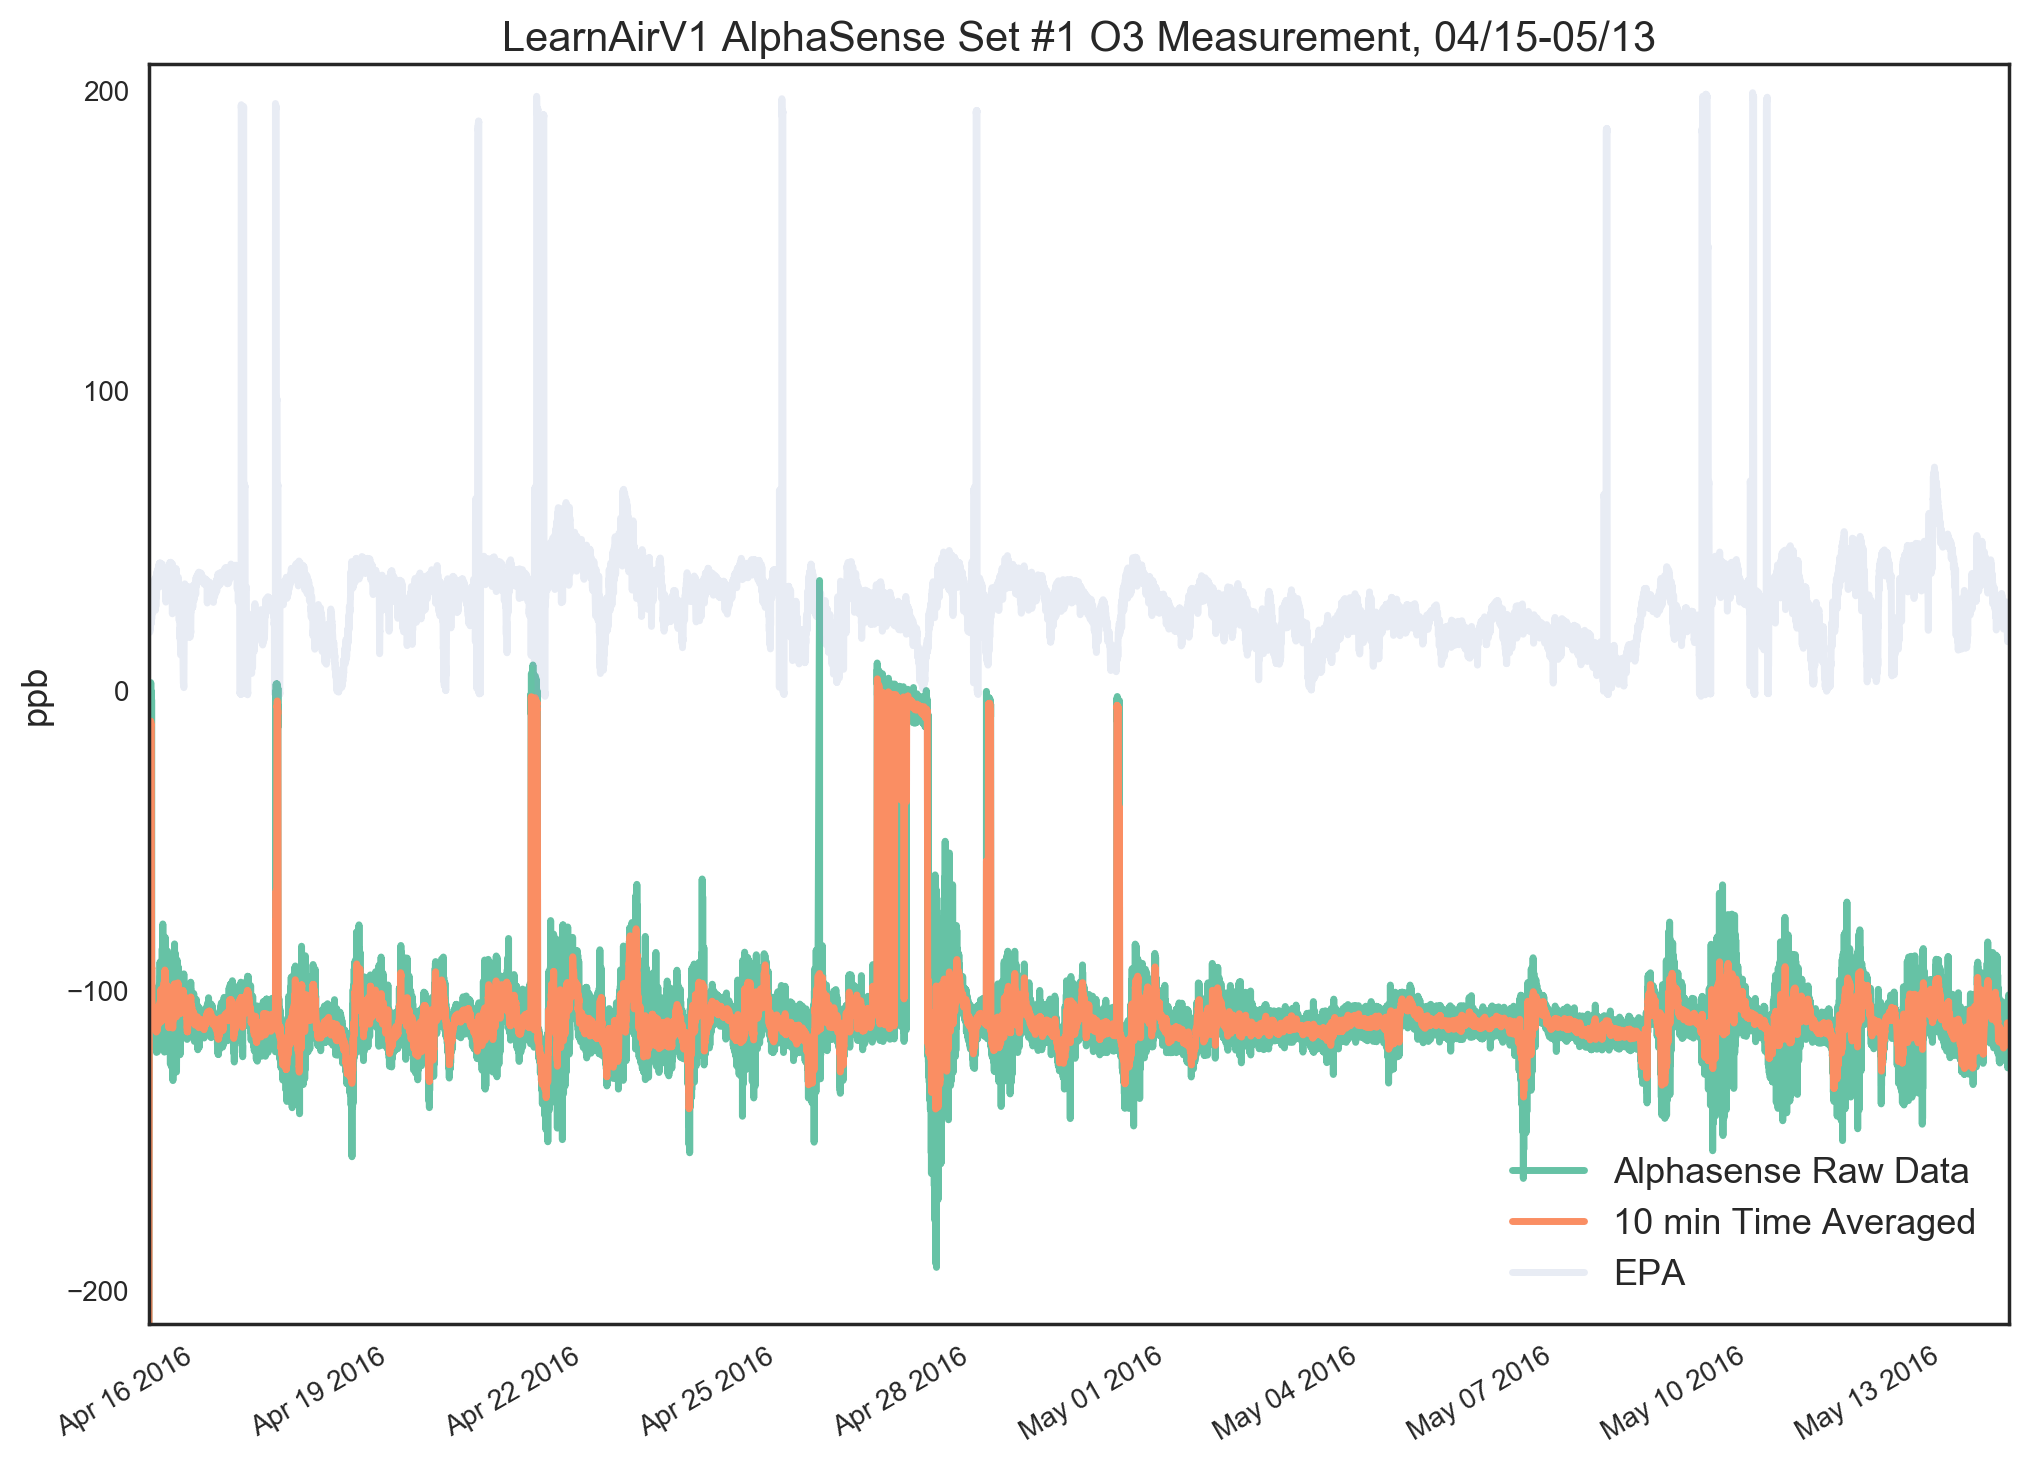
\includegraphics[width=\textwidth]{figs/as1_o3_raw}               
 	 \caption{AlphaSense O3 Sensor #1 Raw Data}
  	\label{fig:as1_o3_raw}
\end{figure}

\begin{figure}[htb]
 	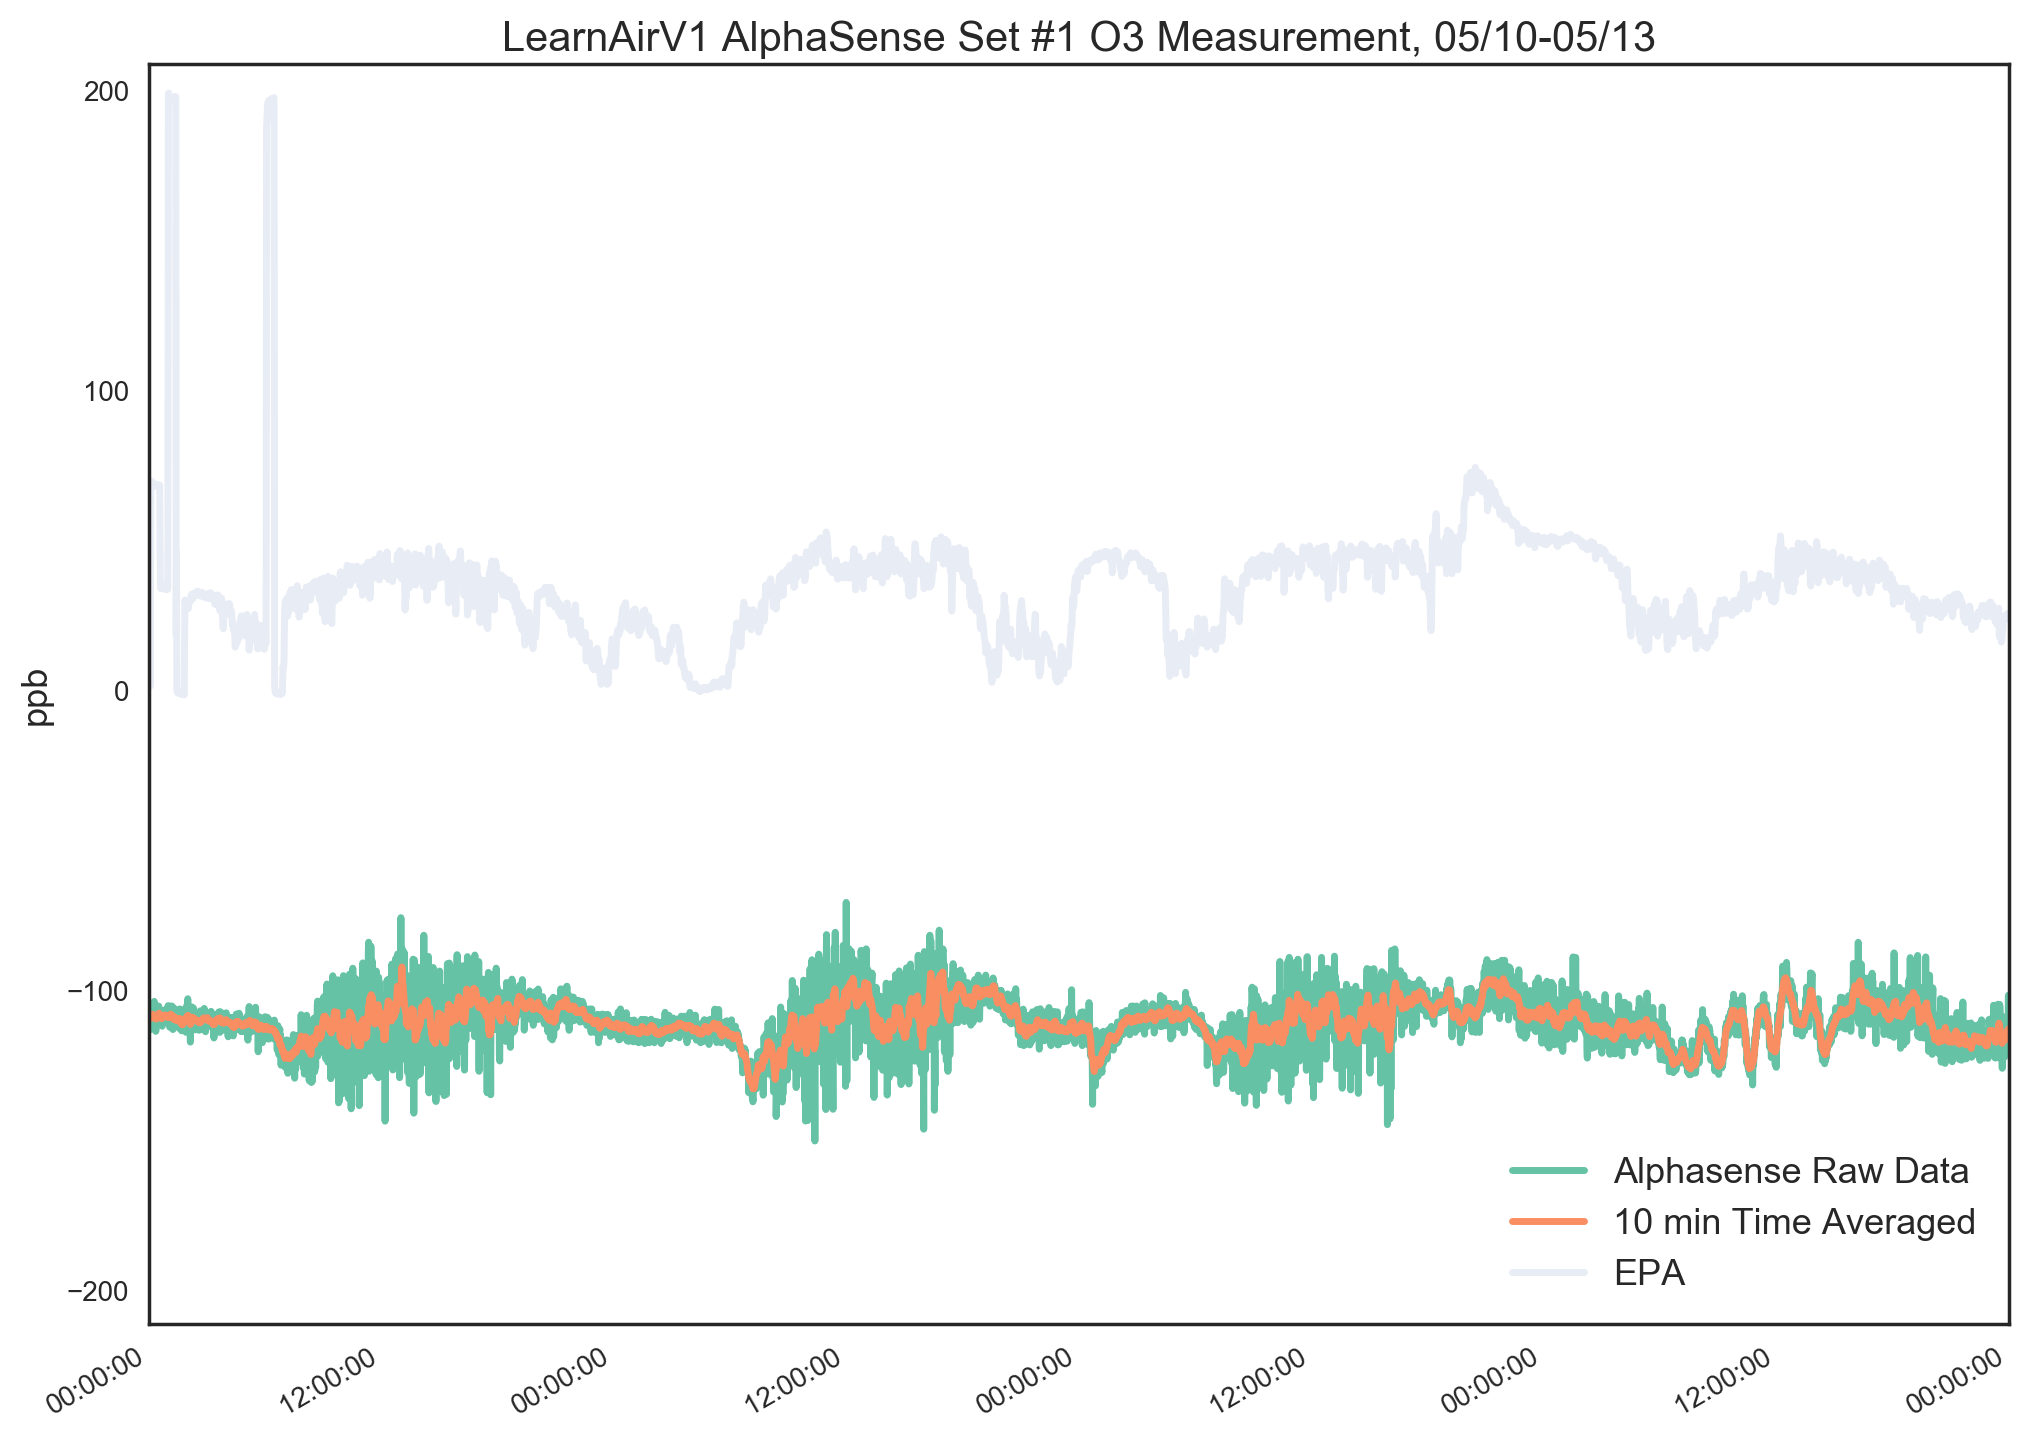
\includegraphics[width=\textwidth]{figs/as1_o3_raw_zoomed}               
 	 \caption{AlphaSense O3 Sensor #1 Raw Data Zoomed}
  	\label{fig:as1_o3_raw_zoomed}
\end{figure}

New sensor all over the map with datasheet calibration because of NO2 calibration using raw calibration values and readings.

\begin{figure}[htb]
 	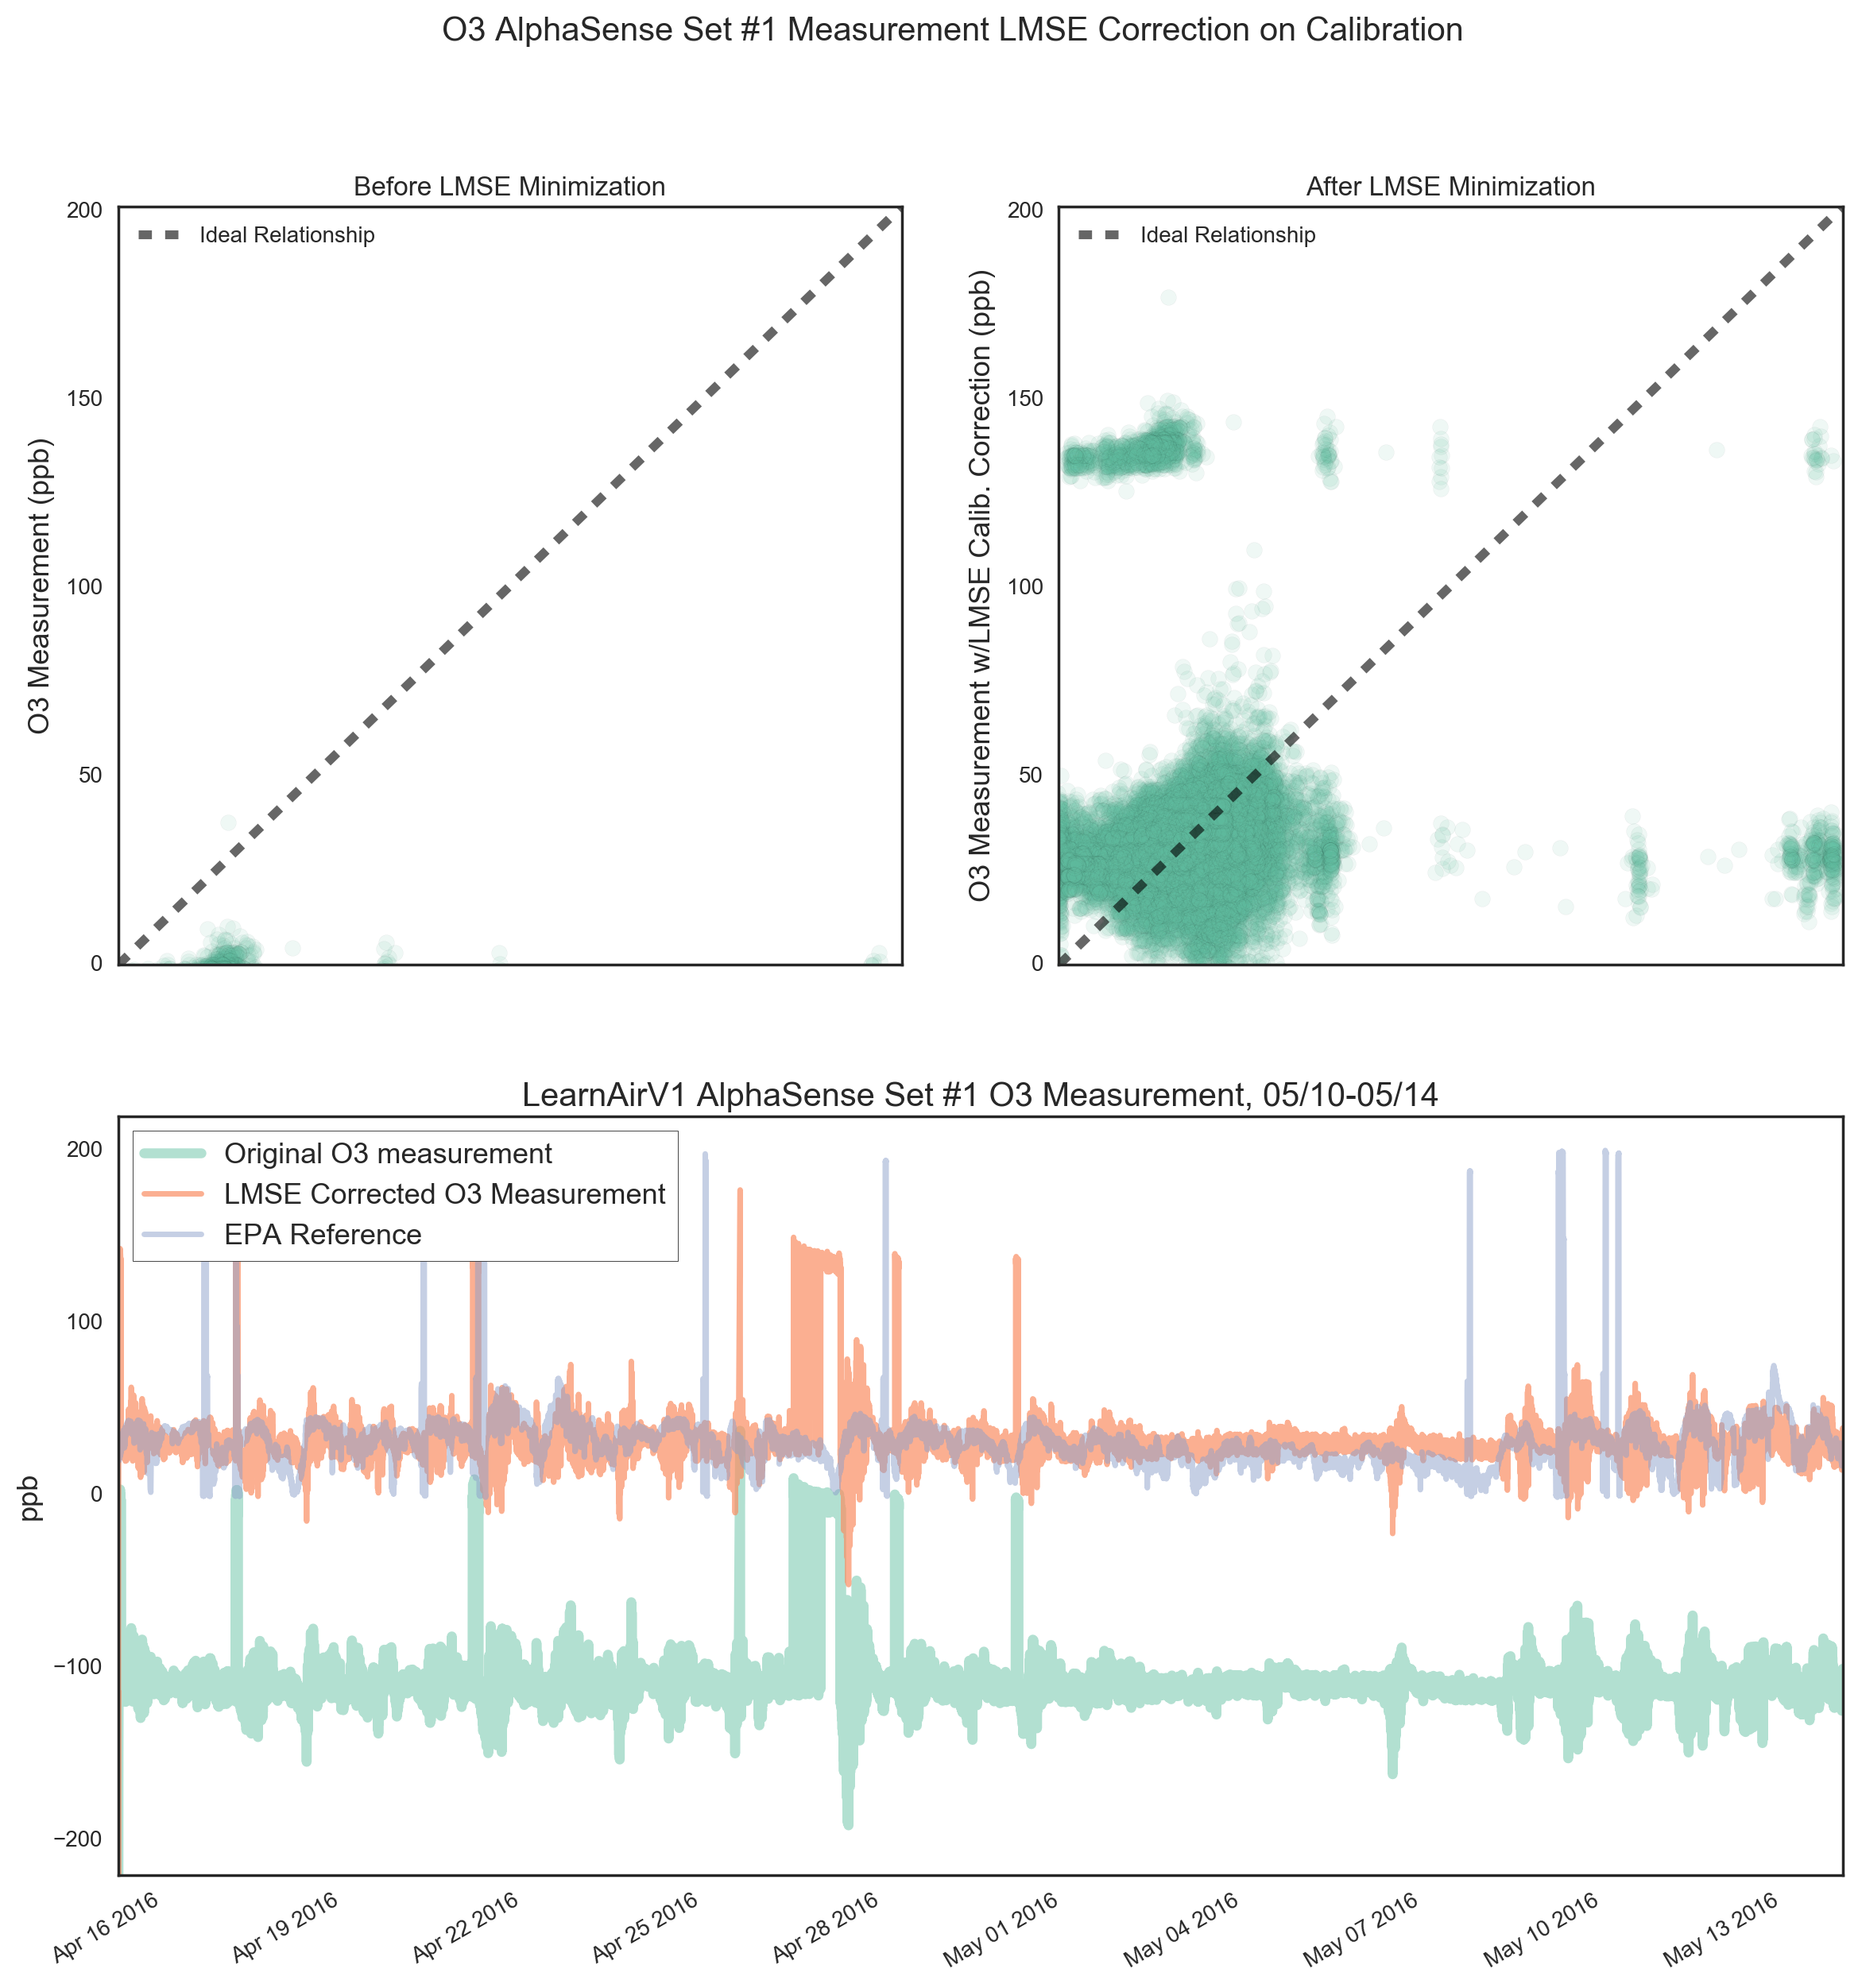
\includegraphics[width=\textwidth]{figs/as1_o3_lmse}               
 	 \caption{AlphaSense O3 Sensor #1 after LMSE Calibration}
  	\label{fig:as1_o3_lmse}
\end{figure}

\begin{figure}[htb]
 	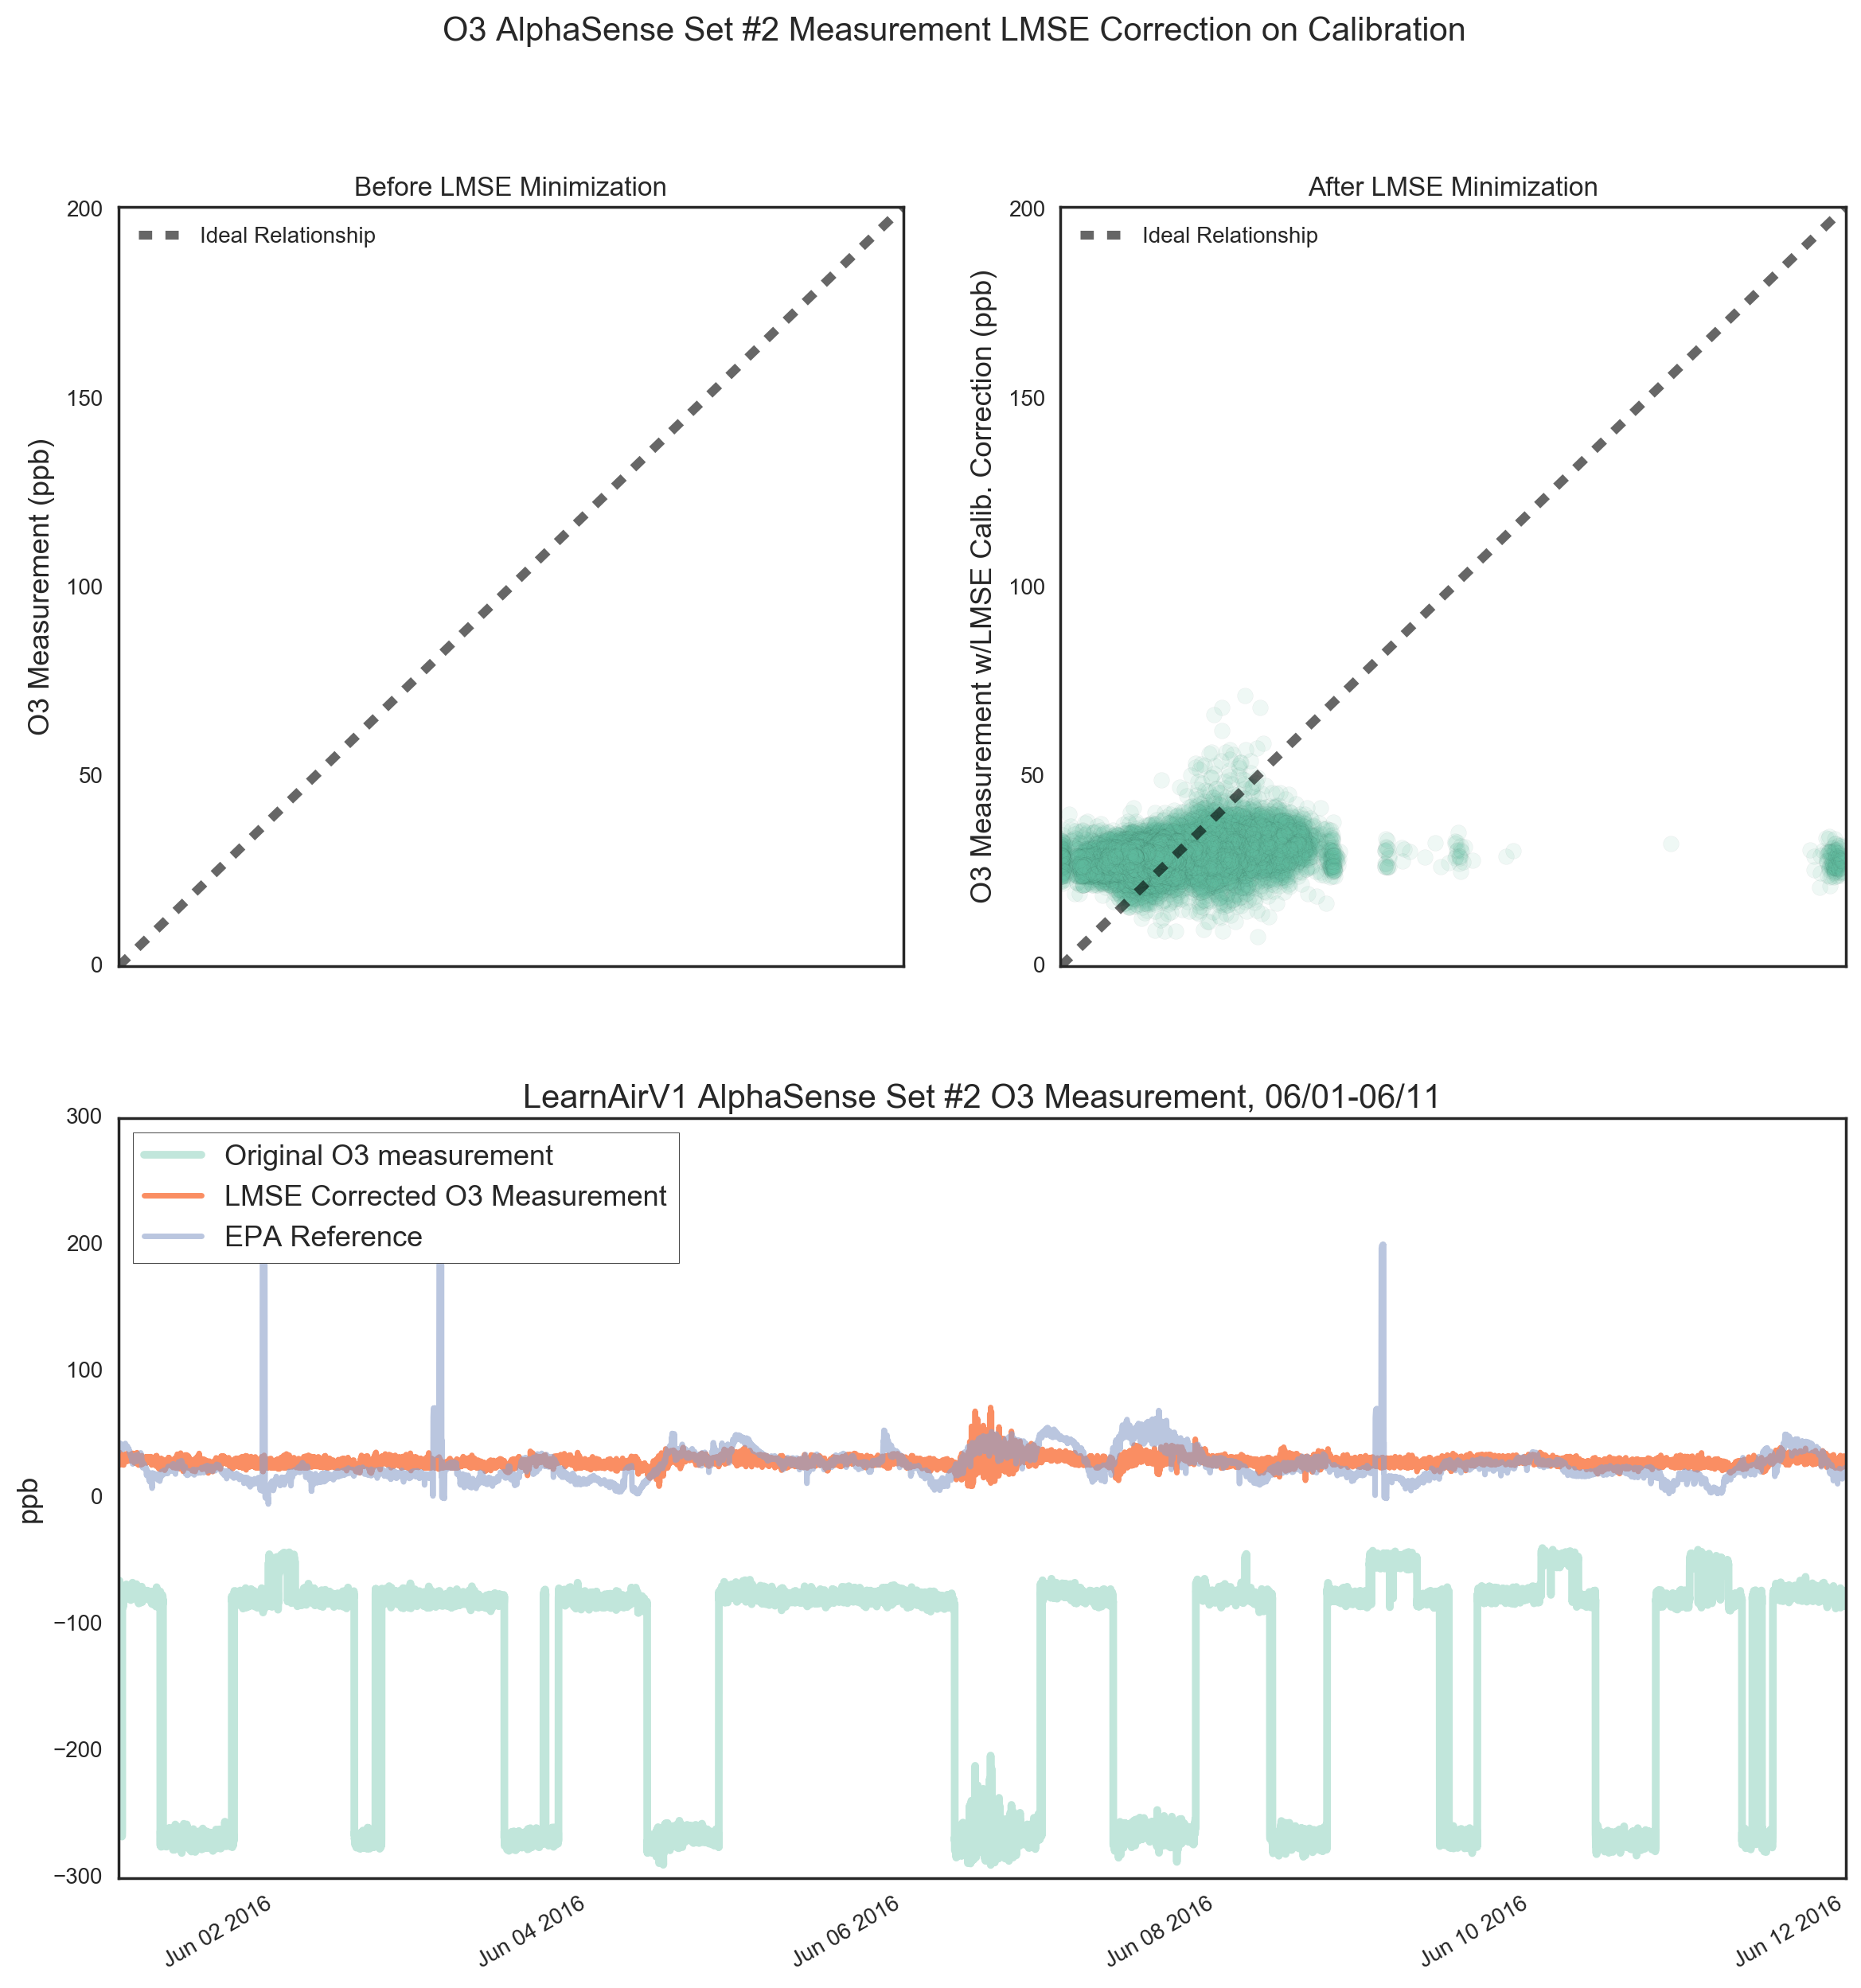
\includegraphics[width=\textwidth]{figs/as2_o3_lmse}               
 	 \caption{AlphaSense O3 Sensor #2 after LMSE Calibration}
  	\label{fig:as2_o3_lmse}
\end{figure}

\subsection{Machine Learning}


\begin{figure}[htb]
 	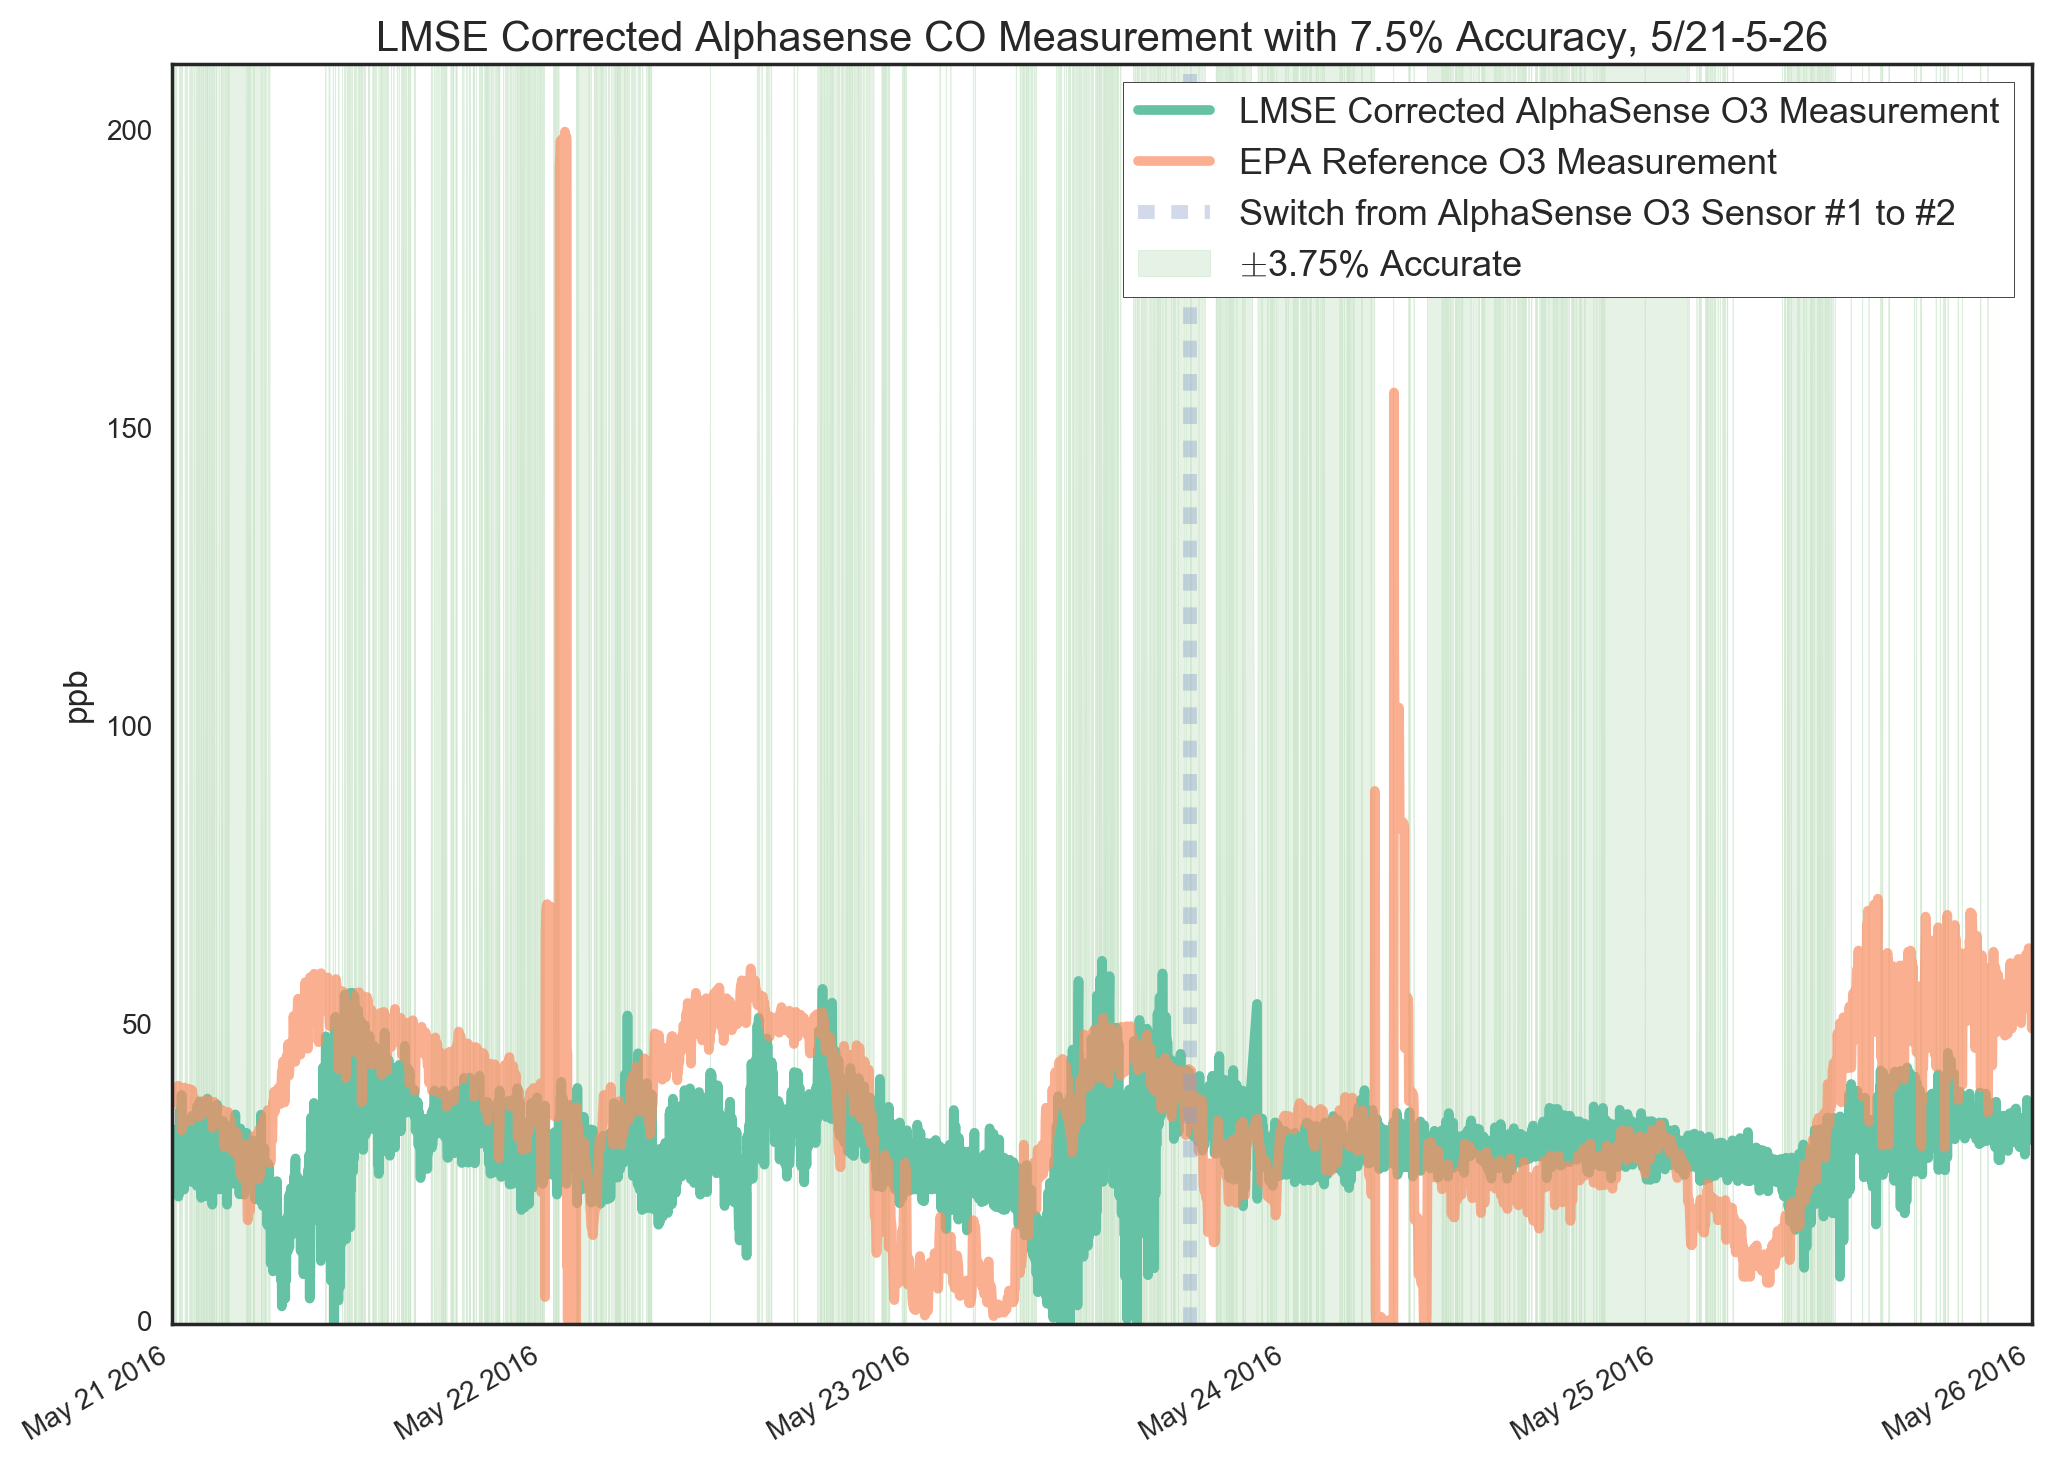
\includegraphics[width=\textwidth]{figs/as_o3_with_7p5_accuracy_zoomed}               
 	 \caption{AlphaSense O3 Sensor #1 and #2 with 7.5\% Accuracy Threshold}
  	\label{fig:as_o3_with_7p5_accuracy_zoomed}
\end{figure}

\begin{figure}[htb]
 	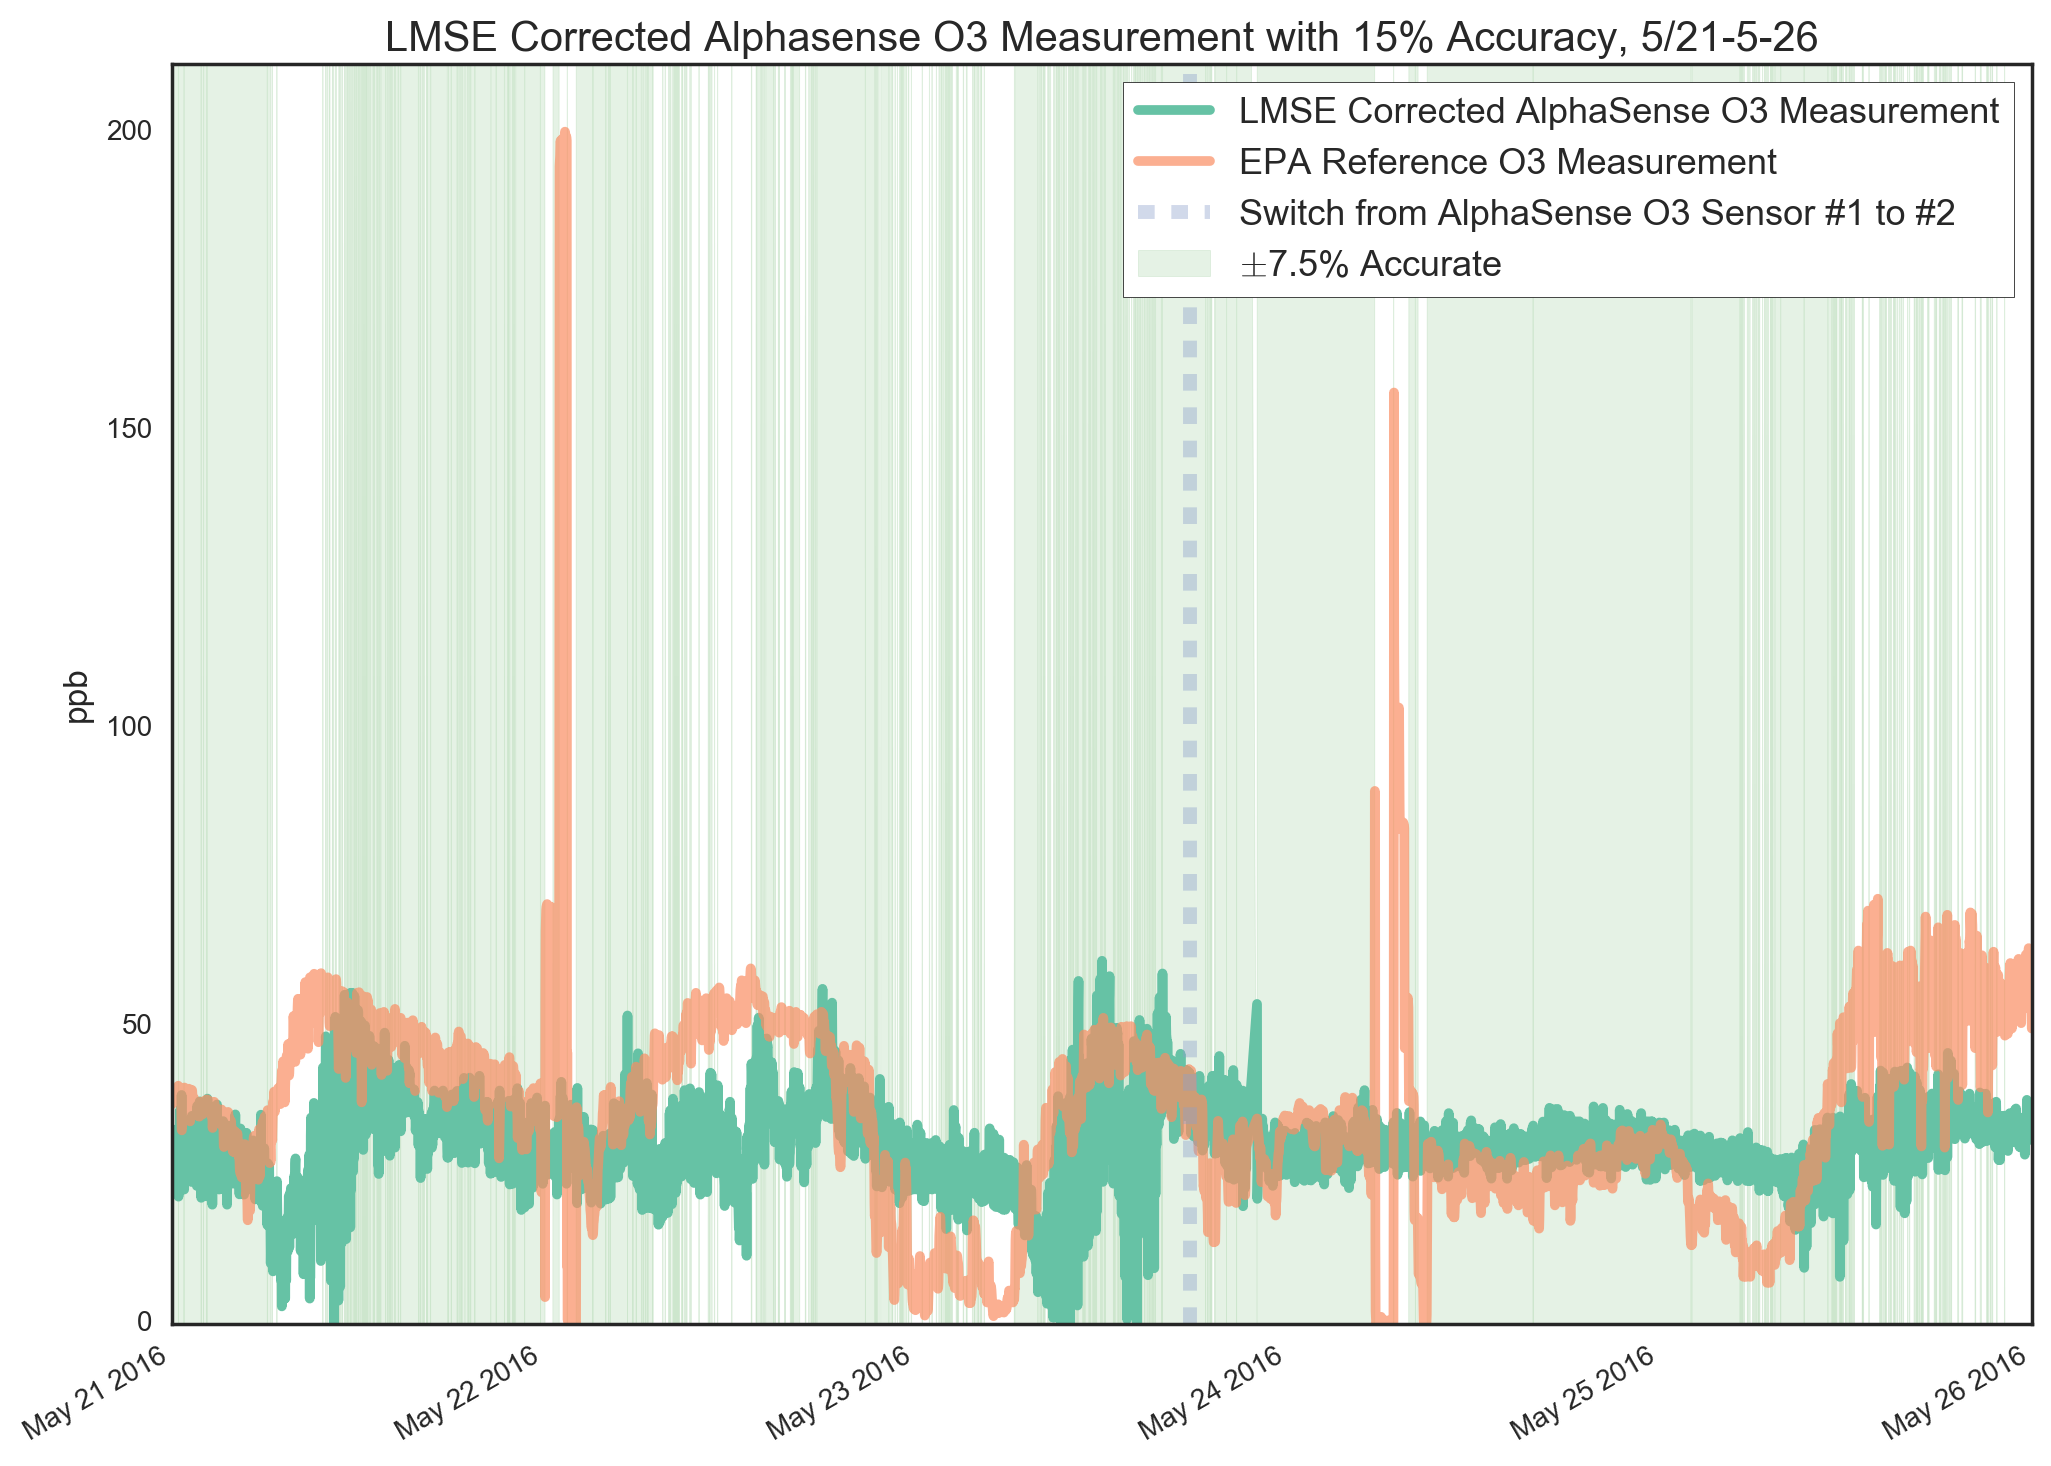
\includegraphics[width=\textwidth]{figs/as_o3_with_5_accuracy_zoomed}               
 	 \caption{AlphaSense O3 Sensor #1 and #2 with 5\% Accuracy Threshold}
  	\label{fig:as_o3_with_5_accuracy_zoomed}
\end{figure}









parameters = {'C':[0.001, 0.1, 10, 1000], 'penalty':('L1', 'L2') }, 2-Fold cross validation

===== best ROC\_AUC score 0.725924836928

===== best params {'penalty': 'L1', 'C': 10}



\begin{table}[H]
\centering
\begin{tabular}{|c|c|c|c|c|}
\toprule
\multicolumn{5}{|c|}{Error Rates for O3 Sensor #1 with Logistic Regression} \\
&\multicolumn{2}{|c|}{all features} & \multicolumn{2}{|c|}{top 15 features} \\
&shuffled & chunked & shuffled & chunked \\
avg & 0.33 & 0.43 & 0.37 & 0.41 \\
min & 0.32 & 0.37 & 0.36 & 0.36 \\
max & 0.33 & 0.52 & 0.37 & 0.52 \\
\bottomrule
\end{tabular}
\label{tab:as1_o3_error_rates}
\caption{Error Rates for Predicting O3 Sensor #1 Accuracy with Logistic Regression}
\end{table}



\begin{table}[H]
\centering
\offinterlineskip
\hspace*{-5cm}\raisebox{-3.5cm}[0pt][0pt]{\rotatebox[origin=c]{90}{\parbox[c][0pt][c]{3cm}{\textbf{Actual Values}\\[20pt]}}}\par
\hspace*{1cm}\MyHBox[\dimexpr5.1cm+6\fboxsep\relax]{Predicted Values}\par
\hspace*{1cm}\MyHBox{0}\MyHBox{1}\par
\MyTBox{0}{4308.2}{1730.2}
\MyTBox{1}{1931.8}{3147.6}
}
\label{tab:as1_o3_confusion}
\caption{AlphaSense O3 Sensor #1 Confusion Matrix w/Shuffled K-Fold}
\end{table}



\begin{figure}[htb]
 	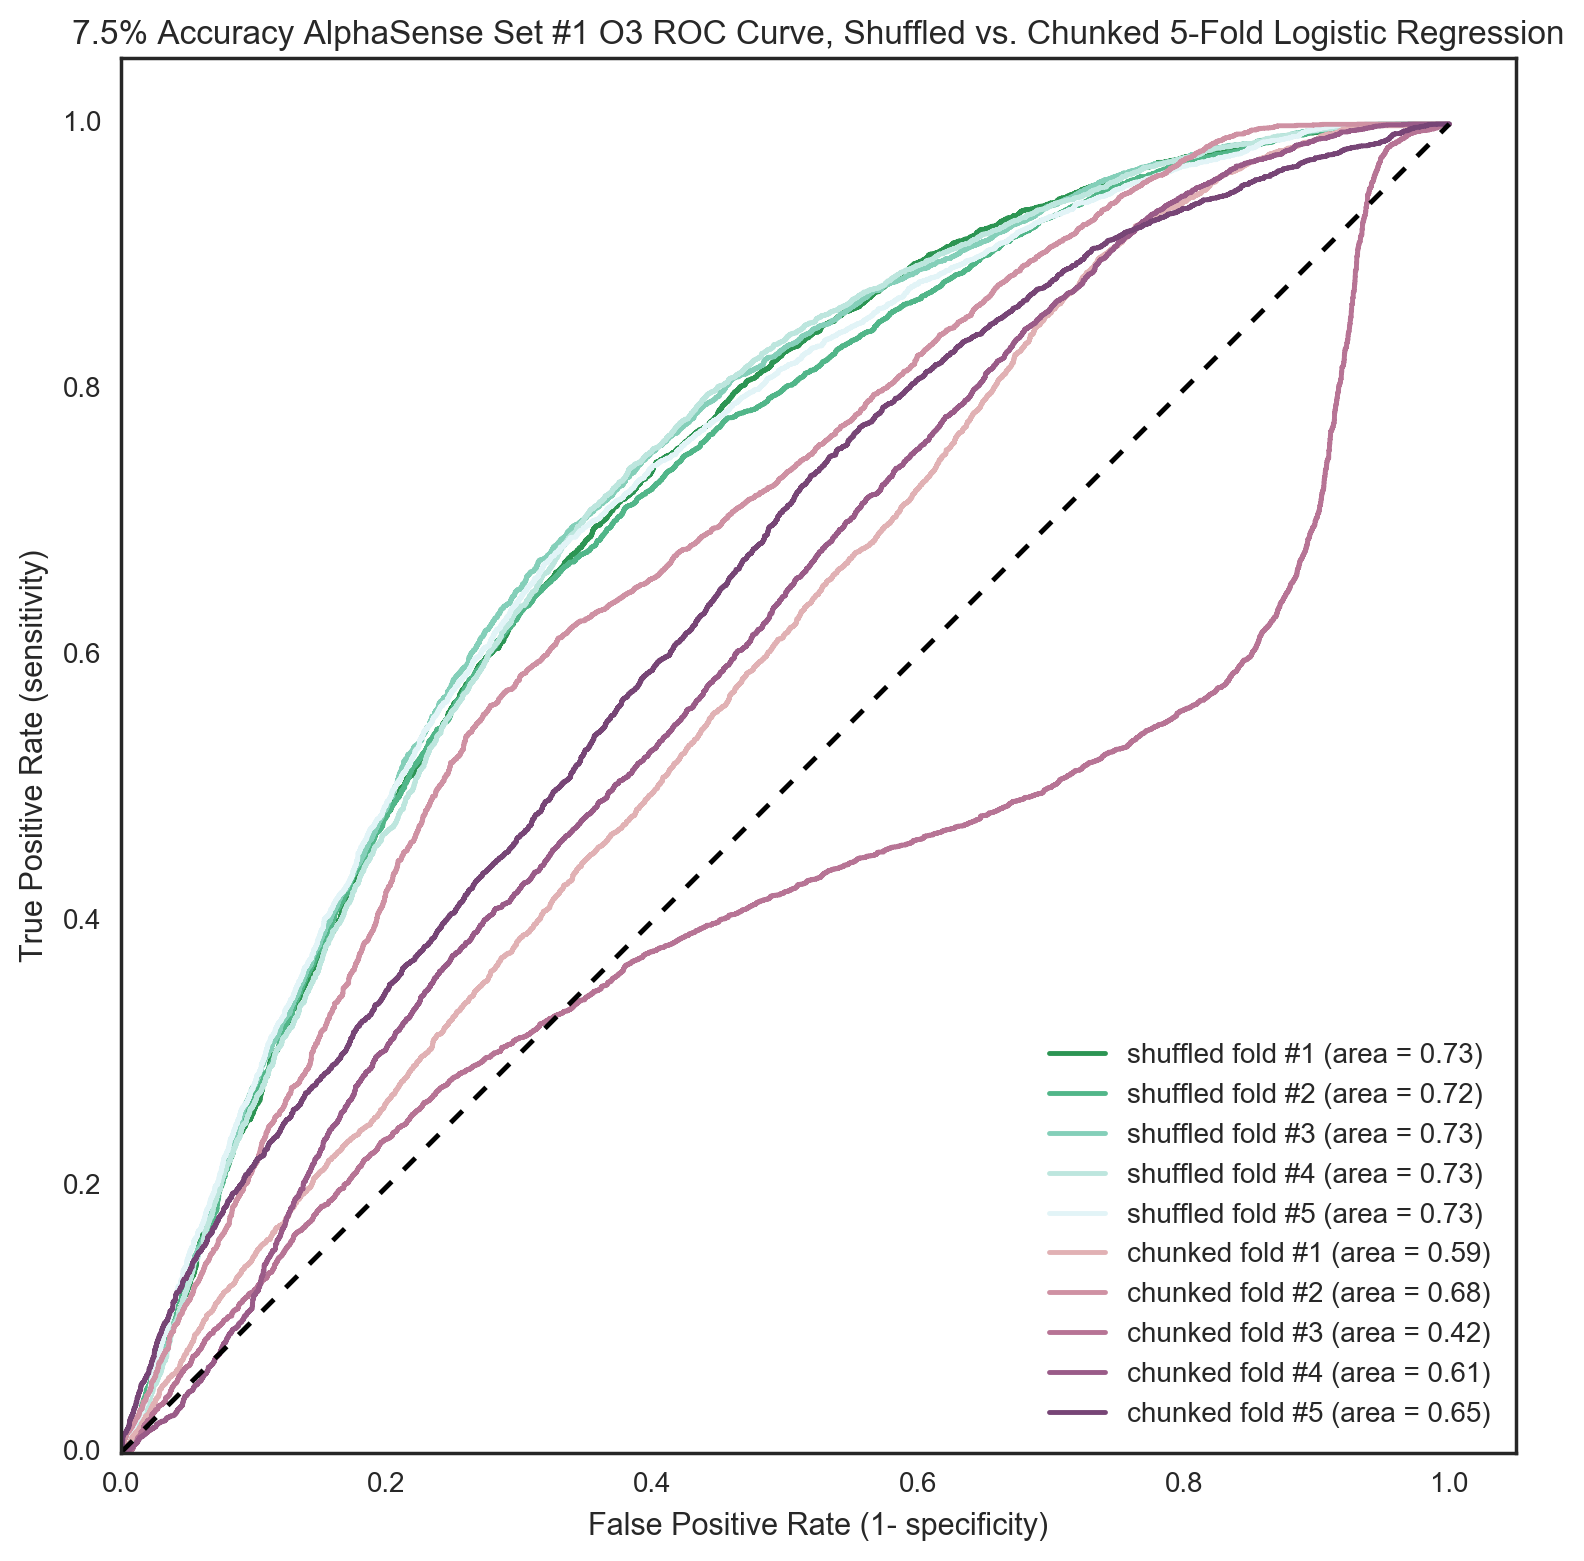
\includegraphics[width=\textwidth]{figs/as1_o3_7p5_roc}               
 	 \caption{AlphaSense O3 Sensor #1 ROC Curve}
  	\label{fig:as1_o3_7p5_roc}
\end{figure}



here's text referencing the (Table \ref{tab:as1_o3_randomforest_features}).

\begin{table}[h]
\centering
\begin{tabular}{lclc|}
\\
\\
\toprule
Feature & Importance \\
\midrule
lmse\_calib\_as\_o3 & 0.0388052728559 \\
as\_o3 & 0.038535780326 \\
alphaS1\_work & 0.0256714422814 \\
avg\_10\_as\_o3 & 0.0143759967966 \\
avg\_10\_lmse\_calib\_as\_o3 & 0.0143305118271 \\
as\_h2s & 0.0131703607364 \\
avg\_720\_bkcarbon & 0.0131177282572 \\
avg\_60\_bkcarbon & 0.0128714271405 \\
avg\_1440\_bkcarbon & 0.0124171125826 \\
min\_since\_plugged\_in & 0.012288250826 \\
bkcarbon & 0.0122005264086 \\
avg\_1440\_lmse\_scaled\_sharpDust & 0.0118815562888 \\
avg\_720\_lmse\_scaled\_sharpDust & 0.0116399996115 \\
daily\_avg\_as\_temperature & 0.0116365039598 \\
alphaS3\_work & 0.0115947138563 \\
\bottomrule
\end{tabular}
\label{tab:as1_o3_randomforest_features}
\caption{Top 15 Features from Random Forest for O3 Sensor #1, used in Pruned Logistic Regression}
\end{table}




\begin{figure}[htb]
 	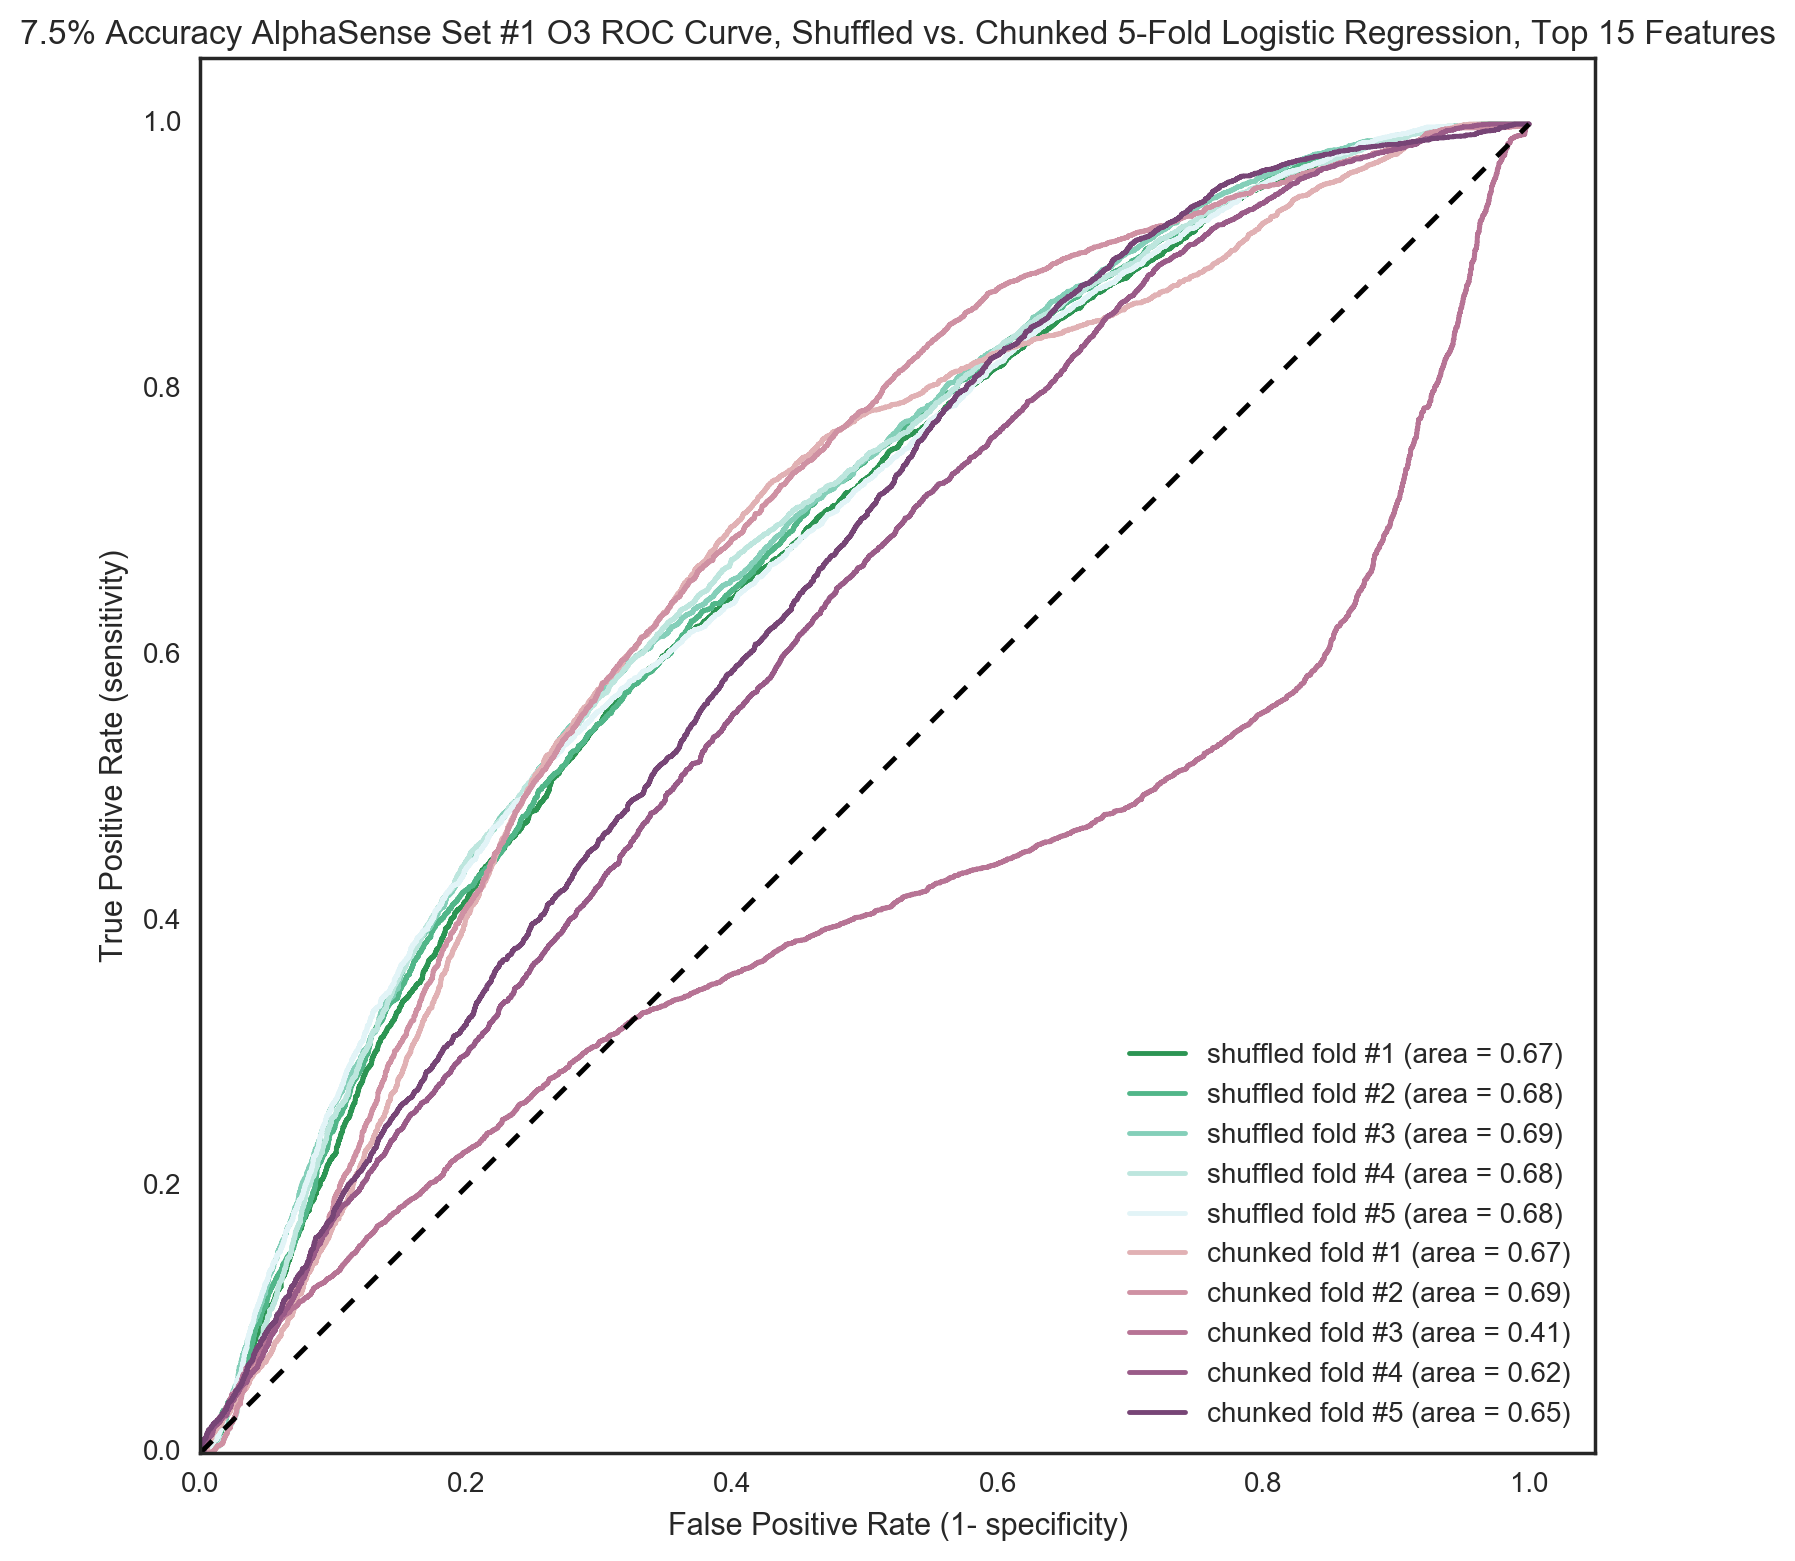
\includegraphics[width=\textwidth]{figs/as1_o3_7p5_roc_pruned_features}               
 	 \caption{AlphaSense O3 Sensor #1 ROC Using Top 15 Features}
  	\label{fig:as1_o3_7p5_roc_pruned_features}
\end{figure}

\begin{figure}[htb]
 	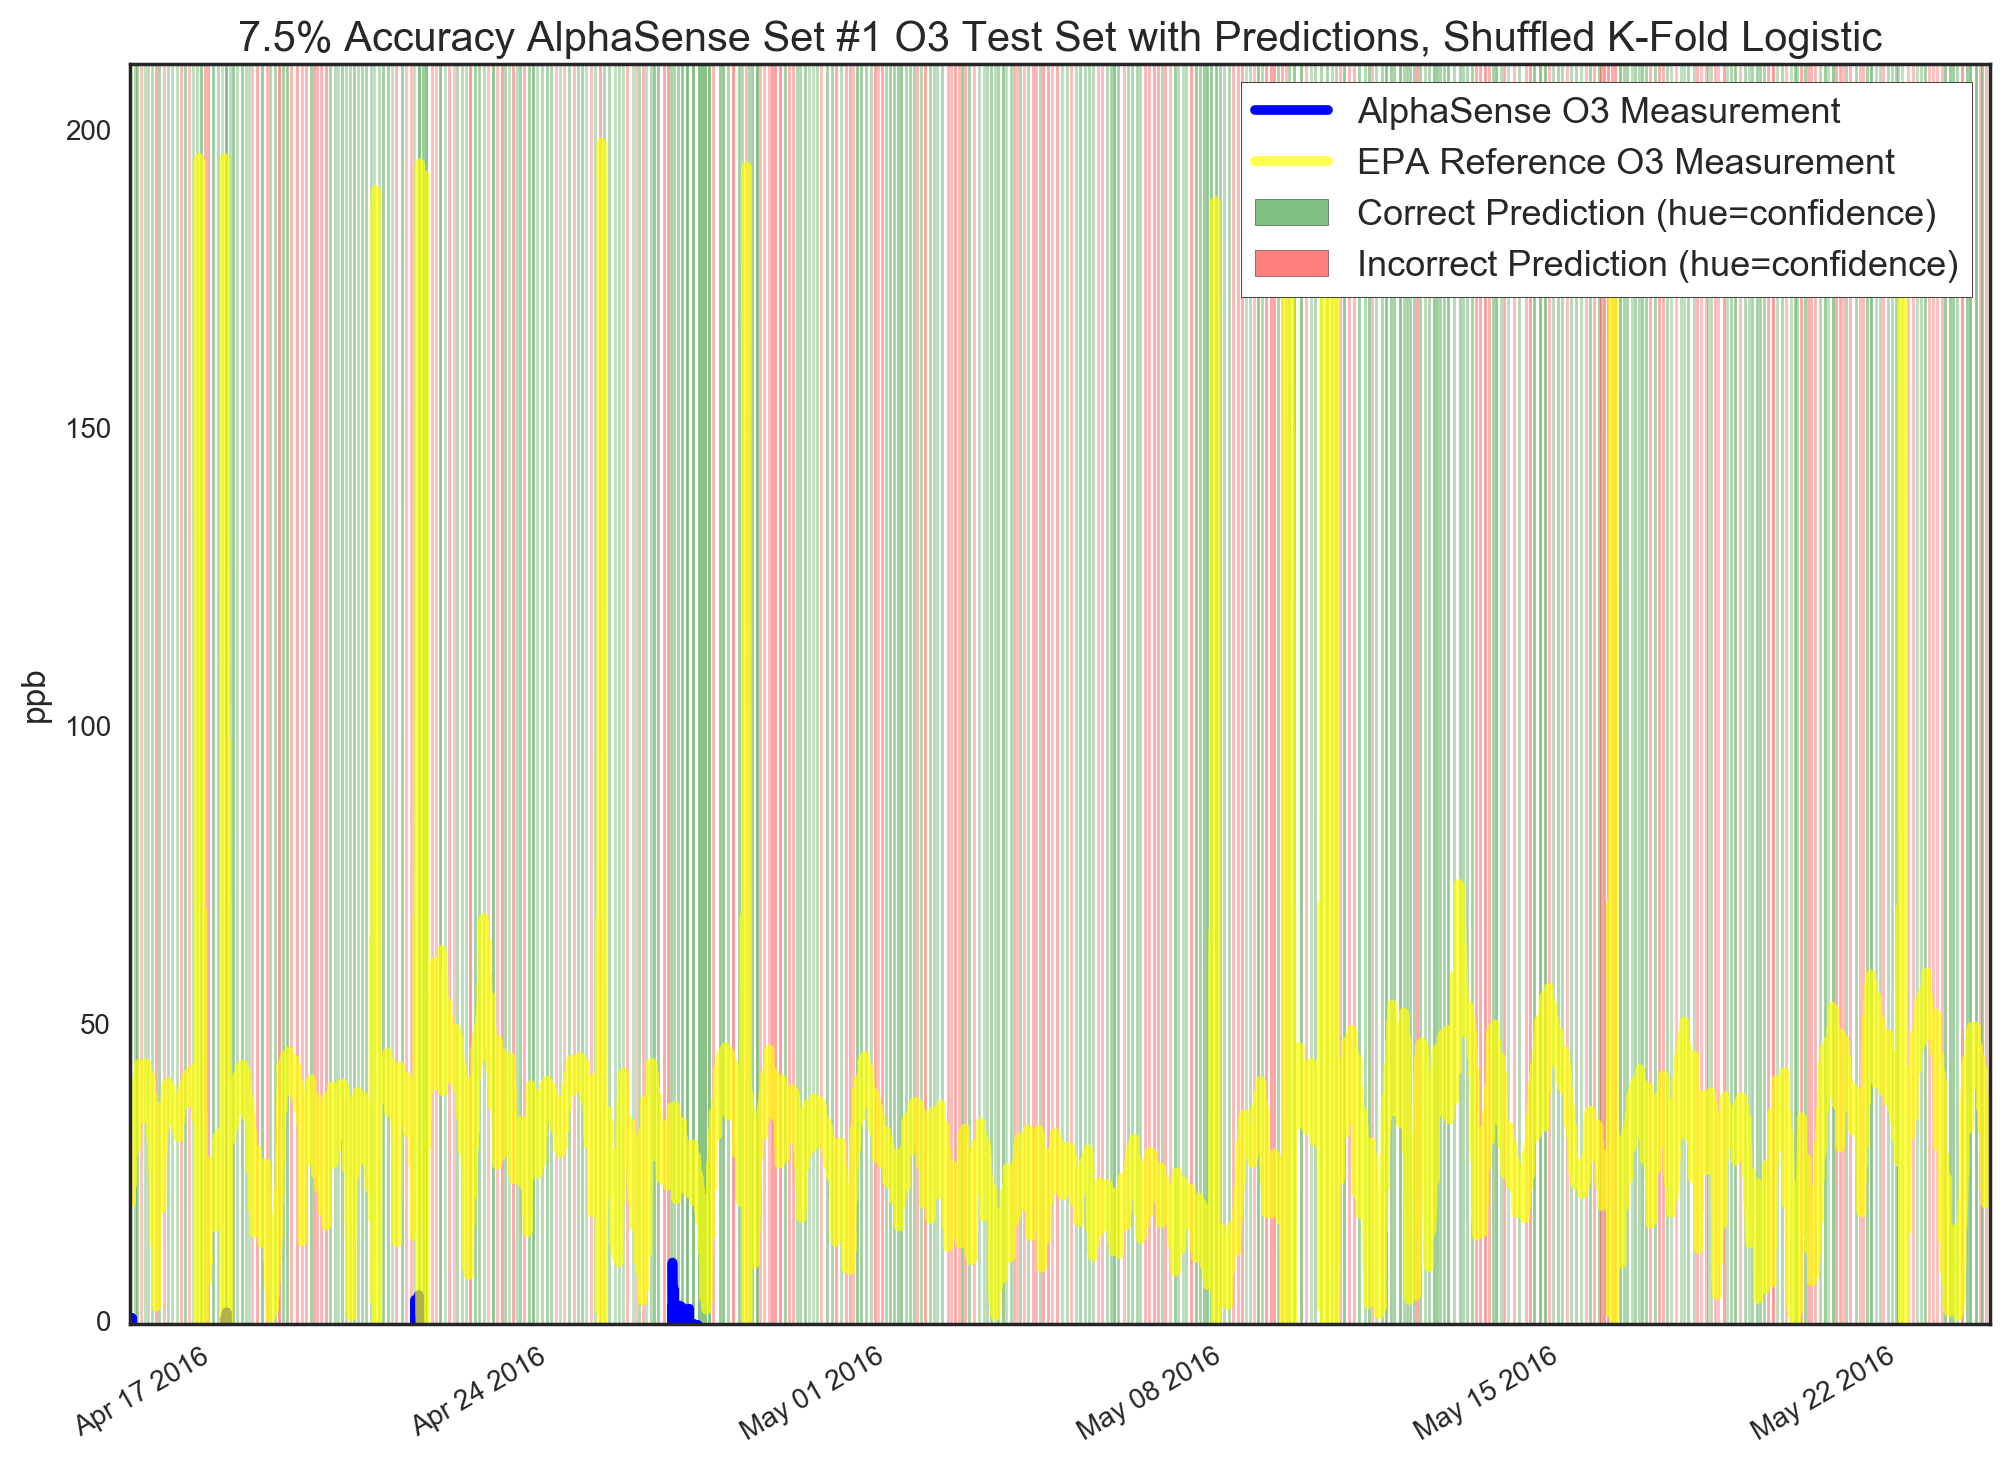
\includegraphics[width=\textwidth]{figs/as1_o3_7p5_logistic_predictions}               
 	 \caption{AlphaSense O3 Sensor #1 Prediction Accuracy}
  	\label{fig:as1_o3_7p5_logistic_predictions}
\end{figure}



here's text referencing the (Table \ref{tab:as1_o3_top_features}).

\begin{table}[H]
\centering
\begin{tabular}{lllllllll}
\\
\\
\toprule
     & Corr. & Lasso & Lin Reg & RF   & RFE  & Ridge & Stability & Mean \\
\midrule
alphaS1\_work                                  & 0.32  & 1     & 0          & 1    & 0.44 & 0.14  & 0.94      & 0.55 \\
as\_h2s                                        & 0.55  & 0.84  & 0          & 0.08 & 0.96 & 0.01  & 0.63      & 0.44 \\
avg\_1440\_lmse\_scaled\_sharpDust             & 0.22  & 0     & 0          & 0.08 & 0.52 & 1     & 1         & 0.4  \\
avg\_720\_bkcarbon                             & 1     & 0     & 0          & 0.24 & 0.54 & 0.27  & 0.59      & 0.38 \\
bkcarbon                                       & 0.97  & 0     & 0          & 0.18 & 0.27 & 0.24  & 0.77      & 0.35 \\
alphaS3\_aux                                   & 0.68  & 0     & 0          & 0.04 & 0.97 & 0.02  & 0.67      & 0.34 \\
forecastio\_windSpeed                          & 0.62  & 0.5   & 0          & 0.07 & 0.29 & 0.03  & 0.75      & 0.32 \\
Solar Panel ( V)                               & 0.17  & 0     & 1          & 0    & 0.98 & 0     & 0         & 0.31 \\
avg\_10\_as\_o3                                & 0.19  & 0.35  & 0          & 0.05 & 0.51 & 0.29  & 0.76      & 0.31 \\
Nitrogen Dioxide ( kOhm)                       & 0.59  & 0.04  & 0          & 0.04 & 0.74 & 0     & 0.67      & 0.3  \\
lmse\_sck\_no2                                 & 0.59  & 0     & 0          & 0.04 & 0.74 & 0     & 0.73      & 0.3  \\
avg\_60\_bkcarbon                              & 0.84  & 0     & 0          & 0.19 & 0.49 & 0.02  & 0.59      & 0.3  \\
derivative\_avg\_1440\_bkcarbon                & 0.19  & 0     & 0          & 0.07 & 0.63 & 0.18  & 1         & 0.3  \\
avg\_1440\_bkcarbon                            & 0.78  & 0     & 0          & 0.25 & 0.53 & 0.36  & 0.01      & 0.28 \\
derivative\_avg\_720\_bkcarbon                 & 0.08  & 0     & 0          & 0.05 & 0.61 & 0.21  & 1         & 0.28 \\
daily\_avg\_forecastio\_humidity               & 0.08  & 0     & 0          & 0.28 & 0.55 & 0.95  & 0.01      & 0.27 \\
avg\_15\_derivative\_avg\_15\_as\_temperature  & 0.3   & 0     & 0          & 0.07 & 0.49 & 0.29  & 0.65      & 0.26 \\
alphaS1\_aux                                   & 0.01  & 0.93  & 0          & 0.06 & 0.45 & 0.13  & 0.17      & 0.25 \\
avg\_60\_forecastio\_temperature\_c            & 0.42  & 0     & 0.01       & 0.07 & 0.76 & 0.01  & 0.48      & 0.25 \\
humidity\_box\_differential                    & 0.15  & 0     & 0.03       & 0.1  & 1    & 0.08  & 0.42      & 0.25 \\
avg\_10\_lmse\_calib\_as\_o3                   & 0.19  & 0     & 0          & 0.04 & 0.51 & 0.29  & 0.7       & 0.25 \\
derivative\_avg\_60\_bkcarbon                  & 0.11  & 0     & 0          & 0.05 & 0.58 & 0.42  & 0.56      & 0.25 \\
derivative\_avg\_1440\_lmse\_scaled\_sharpDust & 0.01  & 0     & 0          & 0.06 & 0.62 & 0.07  & 1         & 0.25 \\
as\_o3                                         & 0.04  & 0     & 0          & 0.76 & 0.79 & 0.01  & 0.07      & 0.24 \\
\bottomrule
\end{tabular}
\label{tab:as1_o3_top_features}
\caption{Top Features for Predicting AlphaSense O3 Sensor #1}
\end{table}








parameters = {'C':[0.001, 0.1, 10, 1000], 'penalty':('L1', 'L2') }, 2-Fold cross validation

===== best ROC\_AUC score 0.816024265233 

===== best params {'penalty': 'L1', 'C': 1000}



\begin{table}[H]
\centering
\begin{tabular}{|c|c|c|c|c|}
\toprule
\multicolumn{5}{|c|}{Error Rates for O3 Sensor #2 with Logistic Regression} \\
&\multicolumn{2}{|c|}{all features} & \multicolumn{2}{|c|}{top 15 features} \\
&shuffled & chunked & shuffled & chunked \\
avg & 0.26 & 0.46 & 0.32 & 0.40 \\
min & 0.24 & 0.37 & 0.32 & 0.35 \\
max & 0.26 & 0.54 & 0.33 & 0.49 \\
\bottomrule
\end{tabular}
\label{tab:as2_o3_error_rates}
\caption{Error Rates for Predicting O3 Sensor #2 Accuracy with Logistic Regression}
\end{table}



\begin{table}[H]
\centering
\offinterlineskip
\hspace*{-5cm}\raisebox{-3.5cm}[0pt][0pt]{\rotatebox[origin=c]{90}{\parbox[c][0pt][c]{3cm}{\textbf{Actual Values}\\[20pt]}}}\par
\hspace*{1cm}\MyHBox[\dimexpr5.1cm+6\fboxsep\relax]{Predicted Values}\par
\hspace*{1cm}\MyHBox{0}\MyHBox{1}\par
\MyTBox{0}{2439.6}{747.4}
\MyTBox{1}{792.2}{2050.8}
}
\label{tab:as2_o3_confusion}
\caption{AlphaSense O3 Sensor #2 Confusion Matrix w/Shuffled K-Fold}
\end{table}



\begin{figure}[htb]
 	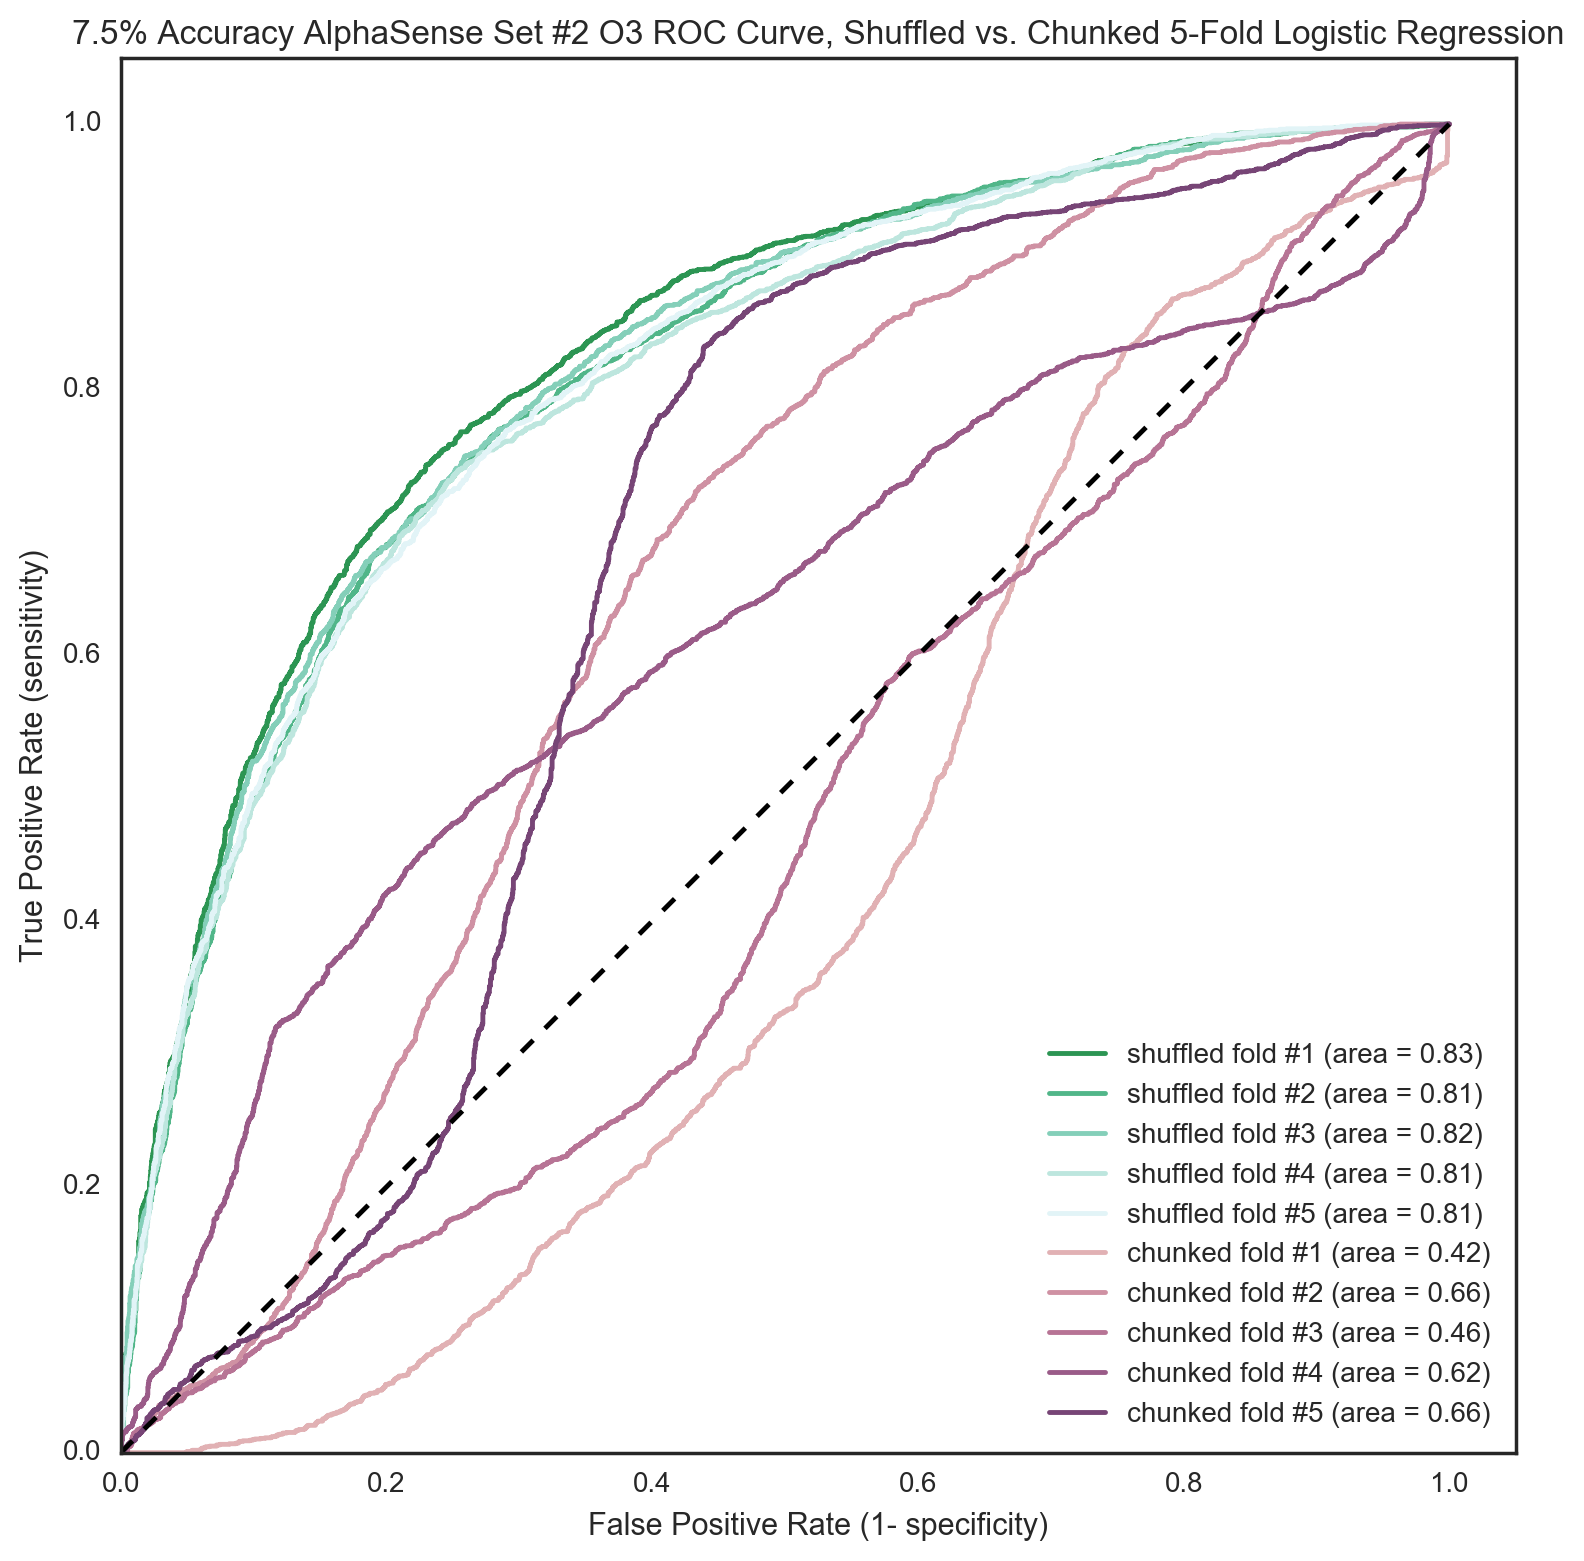
\includegraphics[width=\textwidth]{figs/as2_o3_7p5_roc}               
 	 \caption{AlphaSense O3 Sensor #2 ROC Curve}
  	\label{fig:as2_o3_7p5_roc}
\end{figure}



here's text referencing the (Table \ref{tab:as2_o3_randomforest_features}).

\begin{table}[H]
\centering
\begin{tabular}{lllllllll}
\\
\\
\toprule
Feature & Importance \\
\midrule
avg\_720\_bkcarbon & 0.0190323311421 \\
avg\_1440\_bkcarbon & 0.0186458328226 \\
avg\_1440\_as\_co & 0.0185435347092 \\
daily\_avg\_as\_temperature & 0.0177518437915 \\
lmse\_calib\_as\_o3 & 0.0170424373503 \\
daily\_avg\_forecastio\_temperature & 0.0170308459472 \\ 
avg\_60\_bkcarbon & 0.0167897682822 \\
min\_since\_plugged_in & 0.0166420124401 \\ 
avg\_60\_forecastio\_pressure & 0.016620265085 \\
bkcarbon & 0.015766200638 \\
daily\_avg\_forecastio\_humidity & 0.0147498428636 \\
avg\_60\_forecastio\_apparentTemperature & 0.0140509238175 \\
forecastio\_pressure & 0.013926105091 \\
avg\_60\_forecastio\_temperature_c & 0.0136171116857 \\
day\_of\_year & 0.0133242379573 \\
\bottomrule
\end{tabular}
\label{tab:as2_o3_randomforest_features}
\caption{Top 15 Features from Random Forest for O3 Sensor #2, used in Pruned Logistic Regression}
\end{table}



\begin{figure}[htb]
 	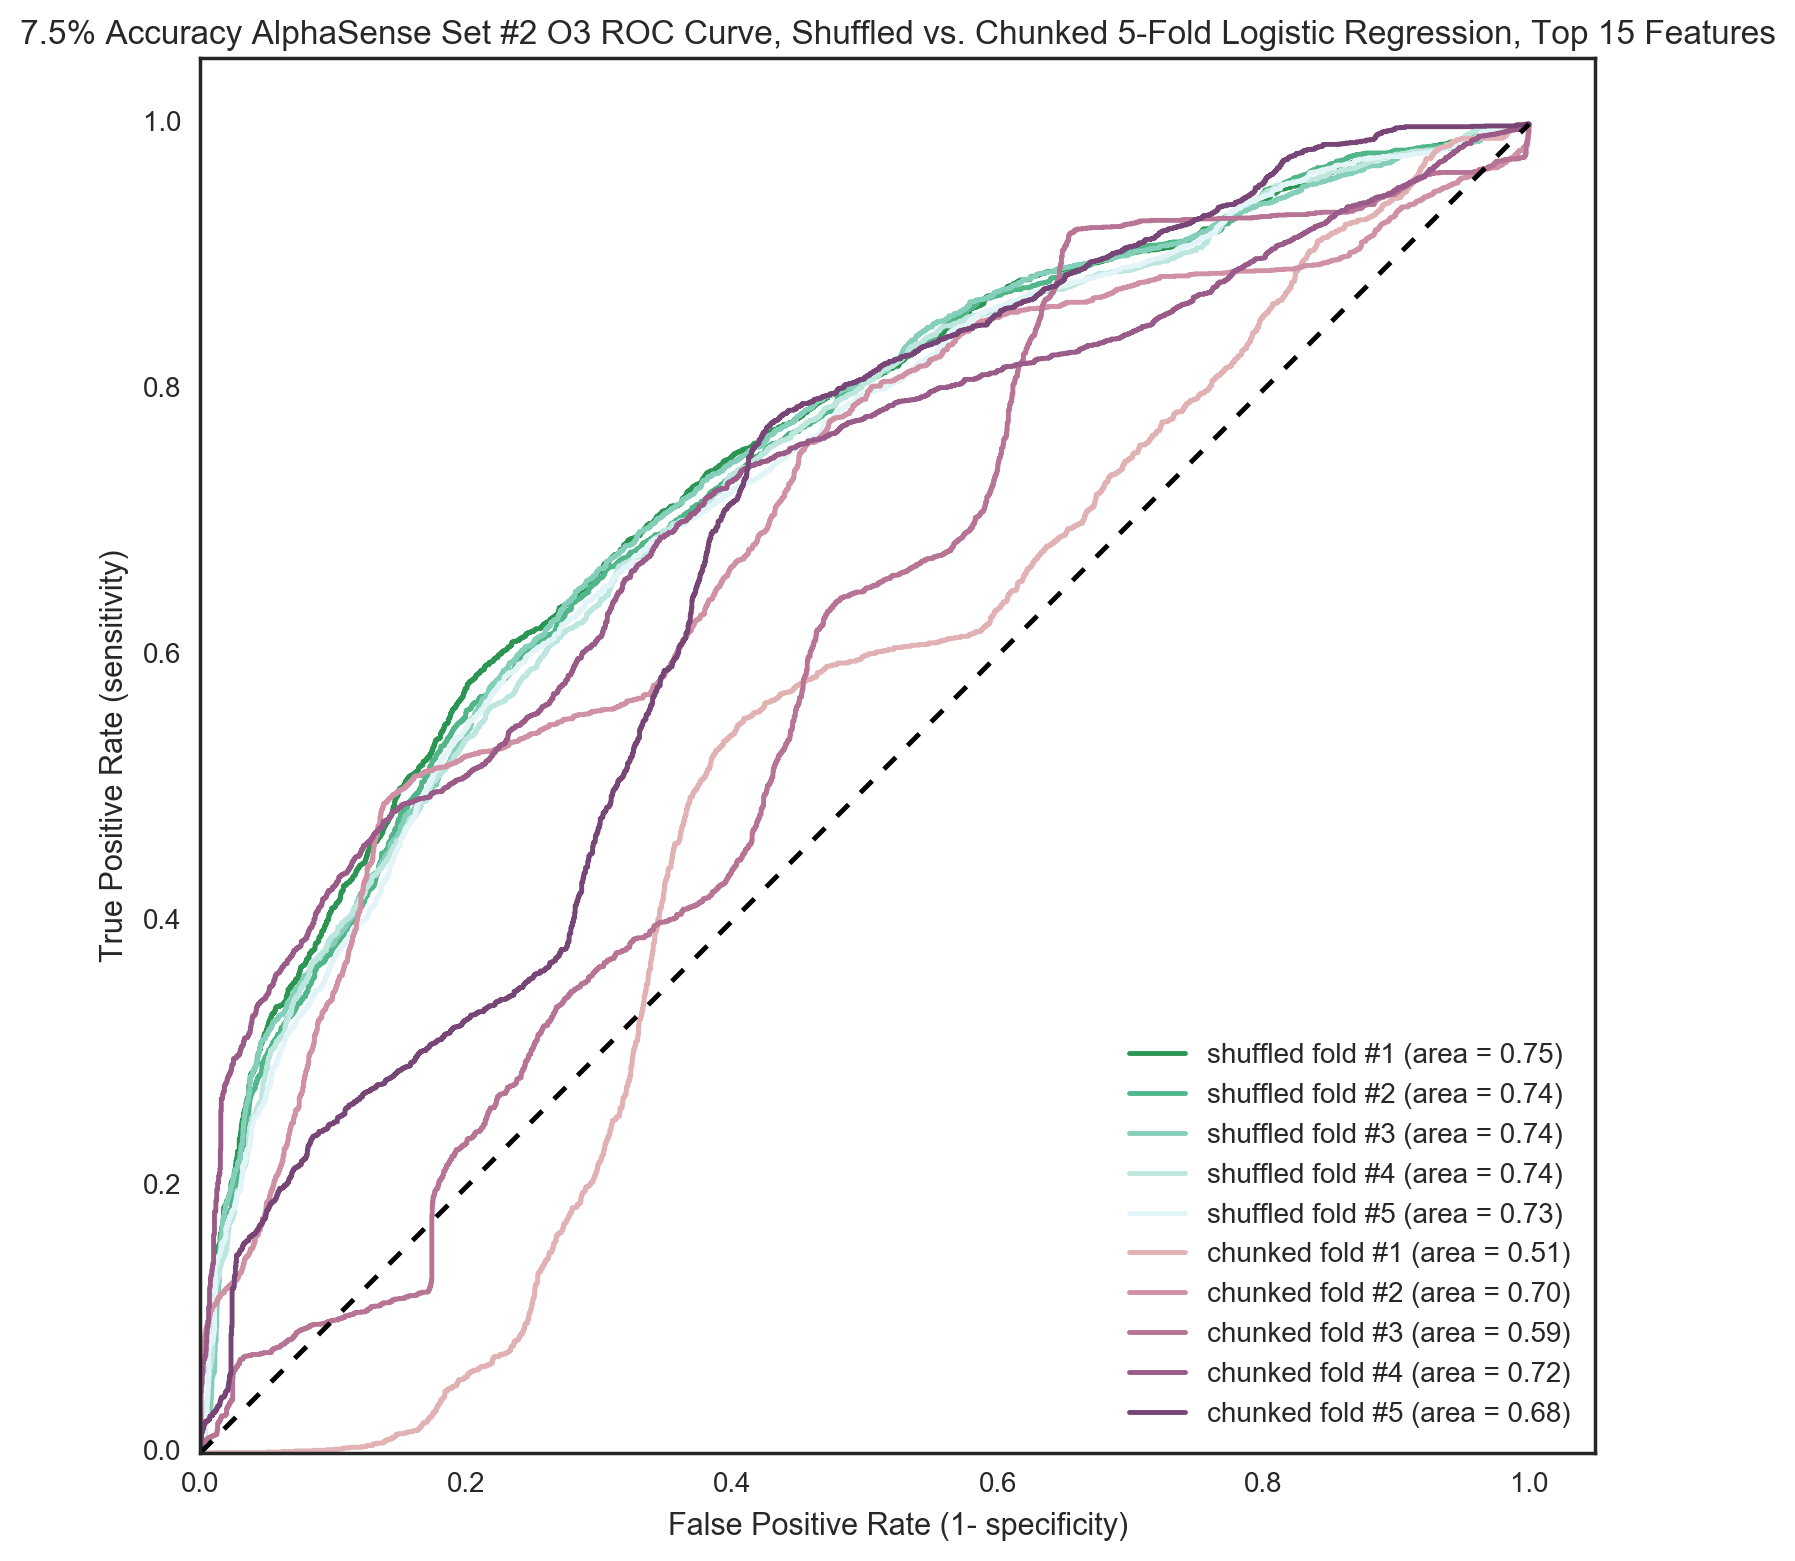
\includegraphics[width=\textwidth]{figs/as2_o3_7p5_roc_pruned_features}               
 	 \caption{AlphaSense O3 Sensor #2 ROC Using Top 15 Features}
  	\label{fig:as2_o3_7p5_roc_pruned_features}
\end{figure}

\begin{figure}[htb]
 	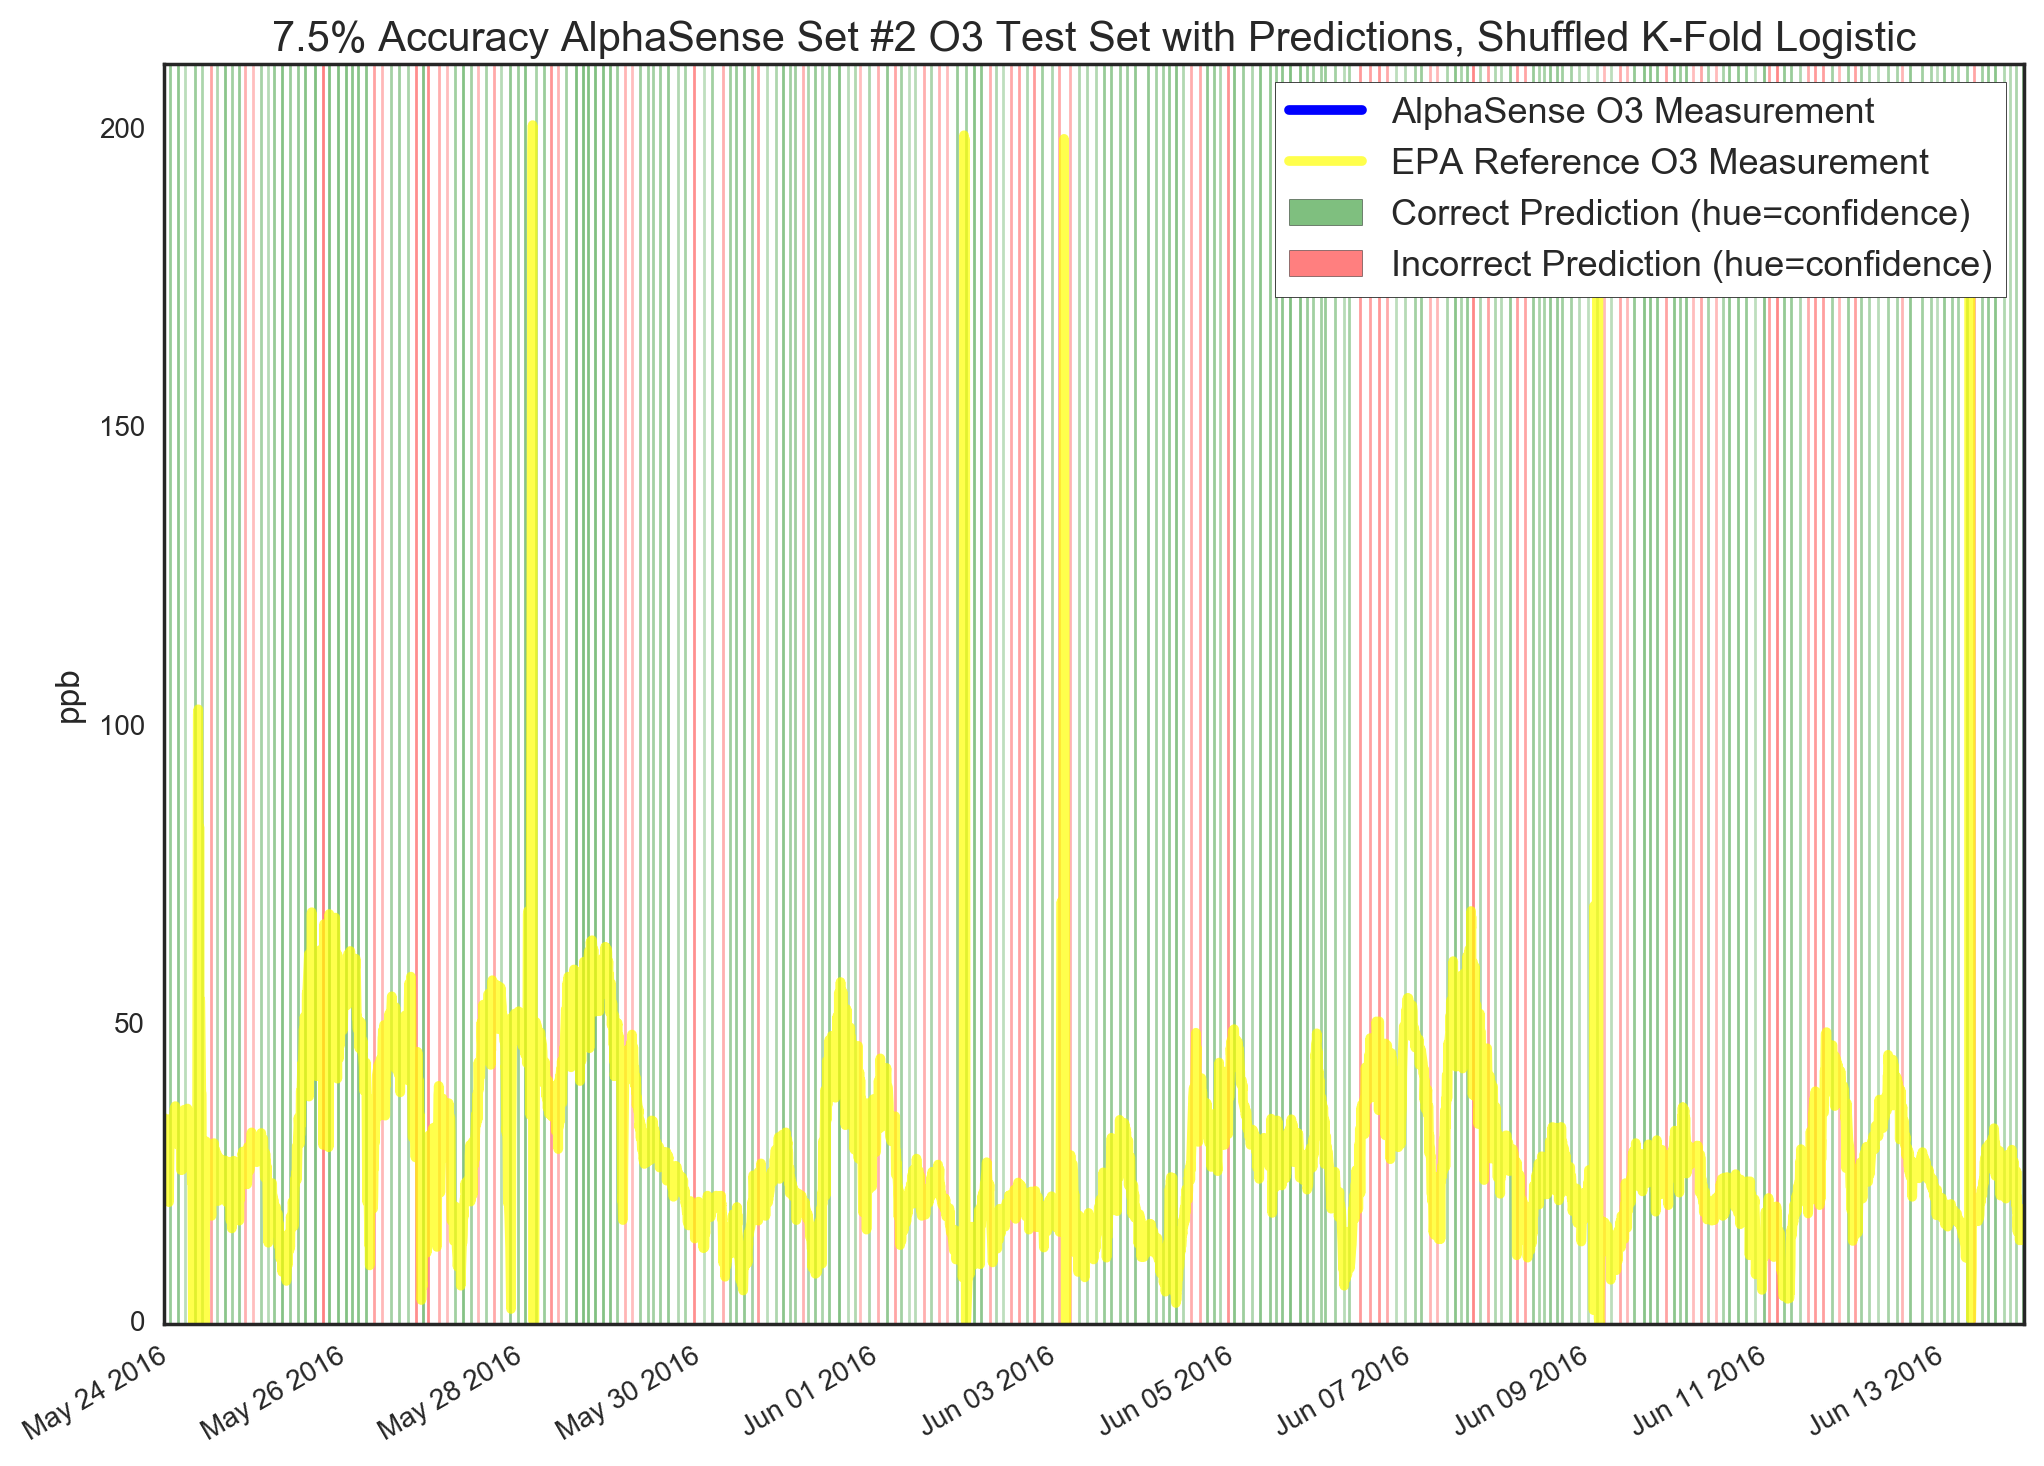
\includegraphics[width=\textwidth]{figs/as2_o3_7p5_logistic_predictions}               
 	 \caption{AlphaSense O3 Sensor #2 Prediction Accuracy}
  	\label{fig:as2_o3_7p5_logistic_predictions}
\end{figure}

\FloatBarrier
here's text referencing the (Table \ref{tab:as2_o3_top_features}).

\begin{table}[!htb]
\centering
\begin{tabular}{lllllllll}
\\
\\
\toprule
     & Corr. & Lasso & Lin Reg & RF   & RFE  & Ridge & Stability & Mean \\
\midrule
avg\_1440\_as\_co                             & 1     & 0.12  & 0          & 0.58 & 0.08 & 0     & 1         & 0.4  \\
daily\_avg\_sck\_humidity                     & 0.71  & 0     & 0          & 0.07 & 0.57 & 1     & 0.36      & 0.39 \\
avg\_1440\_bkcarbon                           & 0.66  & 0     & 0          & 1    & 0.48 & 0.33  & 0.01      & 0.35 \\
avg\_60\_bkcarbon                             & 0.79  & 0     & 0          & 0.38 & 0.35 & 0.06  & 0.8       & 0.34 \\
forecastio\_pressure                          & 0.27  & 0.82  & 0          & 0.1  & 0.33 & 0.04  & 0.75      & 0.33 \\
avg\_60\_forecastio\_apparentTemperature      & 0.17  & 1     & 0          & 0.07 & 0.4  & 0.09  & 0.57      & 0.33 \\
avg\_15\_derivative\_sck\_temperature         & 0.03  & 0     & 0          & 0.04 & 0.57 & 0.45  & 1         & 0.3  \\
bkcarbon                                      & 0.73  & 0     & 0          & 0.14 & 0.47 & 0.04  & 0.66      & 0.29 \\
Solar Panel ( V)                              & 0.1   & 0     & 1          & 0    & 0.86 & 0     & 0         & 0.28 \\
avg\_720\_bkcarbon                            & 0.76  & 0     & 0          & 0.38 & 0.45 & 0.23  & 0.12      & 0.28 \\
derivative\_avg\_1440\_lmse\_calib\_as\_co    & 0.16  & 0     & 0          & 0.08 & 0.51 & 0.14  & 1         & 0.27 \\
daily\_avg\_as\_temperature                   & 0.79  & 0     & 0          & 0.19 & 0.43 & 0.11  & 0.31      & 0.26 \\
lmse\_avg\_30\_scaled\_arduino\_ws            & 0.34  & 0.06  & 0          & 0.04 & 0.94 & 0.01  & 0.4       & 0.26 \\
avg\_1440\_lmse\_scaled\_sharpDust            & 0.05  & 0     & 0          & 0.1  & 0.53 & 0.39  & 0.77      & 0.26 \\
derivative\_avg\_720\_lmse\_scaled\_sharpDust & 0.1   & 0     & 0          & 0.08 & 0.61 & 0.05  & 1         & 0.26 \\
alphaS1\_aux                                  & 0     & 0     & 0.03       & 0.04 & 0.69 & 0.02  & 1         & 0.25 \\
avg\_30\_scaled\_arduino\_ws                  & 0.34  & 0     & 0.01       & 0.04 & 0.95 & 0     & 0.41      & 0.25 \\
derivative\_avg\_1440\_bkcarbon               & 0.09  & 0     & 0          & 0.06 & 0.61 & 0.01  & 1         & 0.25 \\
forecastio\_cloudCover                        & 0.23  & 0     & 0          & 0.16 & 0.49 & 0.01  & 0.64      & 0.22 \\
forecastio\_clear-day                         & 0.01  & 0     & 0.03       & 0    & 0.89 & 0.02  & 0.56      & 0.22 \\
avg\_60\_forecastio\_pressure                 & 0.28  & 0     & 0          & 0.2  & 0.33 & 0.03  & 0.72      & 0.22 \\
Nitrogen Dioxide ( kOhm)                      & 0.1   & 0.13  & 0          & 0.04 & 0.78 & 0     & 0.41      & 0.21 \\
forecastio\_temperature\_c                    & 0.17  & 0     & 0.01       & 0.27 & 0.87 & 0.05  & 0.06      & 0.2  \\
avg\_60\_as\_no2                              & 0.03  & 0.04  & 0          & 0.09 & 0.77 & 0     & 0.47      & 0.2 \\
\bottomrule
\end{tabular}
\label{tab:as2_o3_top_features}
\caption{Top Features for Predicting AlphaSense O3 Sensor #2}
\end{table}



